\documentclass[10pt,landscape,a4paper]{article}
%\usepackage[utf8]{inputenc}
%\usepackage[ngerman]{babel}
\usepackage[normalem]{ulem}
\usepackage{tikz}
\usetikzlibrary{shapes,positioning,arrows,fit,calc,graphs,graphs.standard}
\usepackage[nosf]{kpfonts}
\usepackage[t1]{sourcesanspro}
%\usepackage[lf]{MyriadPro}
%\usepackage[lf,minionint]{MinionPro}
\usepackage{multicol}
\usepackage{wrapfig}
\usepackage[top=0mm,bottom=1mm,left=0mm,right=1mm]{geometry}
\usepackage[framemethod=tikz]{mdframed}
\usepackage{microtype}
%\usepackage{physics}
\usepackage{tabularx}
\usepackage{hhline}
\usepackage{makecell}
\usepackage{mathtools}

\usepackage{listings}

\DeclarePairedDelimiter{\ceil}{\lceil}{\rceil}

\newcommand\codeblue[1]{\textcolor{blue}{\code{#1}}}

\usepackage{lastpage}
\usepackage{datetime}
\yyyymmdddate
\renewcommand{\dateseparator}{-}
\let\bar\overline

\definecolor{myblue}{cmyk}{1,.72,0,.38}

\def\firstcircle{(0,0) circle (1.5cm)}
\def\secondcircle{(0:2cm) circle (1.5cm)}

\colorlet{circle edge}{myblue}
\colorlet{circle area}{myblue!5}

\tikzset{filled/.style={fill=circle area, draw=circle edge, thick},
outline/.style={draw=circle edge, thick}}

\pgfdeclarelayer{background}
\pgfsetlayers{background,main}

%\everymath\expandafter{\the\everymath \color{myblue}}
%\everydisplay\expandafter{\the\everydisplay \color{myblue}}


\renewcommand{\baselinestretch}{.8}
\pagestyle{empty}

\global\mdfdefinestyle{header}{%
  linecolor=gray,linewidth=1pt,%
  leftmargin=0mm,rightmargin=0mm,skipbelow=0mm,skipabove=0mm,
}

\newcommand{\header}{
  \begin{mdframed}[style=header]
    \footnotesize
    \sffamily
    CS2106 Finals Cheatsheet v1.2 (\today)\\
    by~Julius Putra Tanu Setiaji,~page~\thepage~of~\pageref{LastPage}
  \end{mdframed}
}

\let\counterwithout\relax
\let\counterwithin\relax
\usepackage{chngcntr}

\usepackage{verbatim}

\usepackage{etoolbox}
\makeatletter
\preto{\@verbatim}{\topsep=0pt \partopsep=0pt }
\makeatother

\counterwithin*{equation}{section}
\counterwithin*{equation}{subsection}
\usepackage{enumitem}
\newlist{legal}{enumerate}{10}
\setlist[legal]{label*=\arabic*.,leftmargin=2.5mm}
\setlist[itemize]{leftmargin=3mm}
\setlist[enumerate]{leftmargin=3.5mm}
\setlist{nosep}
\usepackage{minted}

\def\code#1{\texttt{#1}}

\newenvironment{descitemize} % a mixture of description and itemize
{\begin{description}[leftmargin=*,before=\let\makelabel\descitemlabel]}
{\end{description}}

\newcommand{\descitemlabel}[1]{%
  \textbullet\ \textbf{#1}%
}
\makeatletter



\renewcommand{\section}{\@startsection{section}{1}{0mm}%
  {.2ex}%
  {.2ex}%x
{\color{myblue}\sffamily\small\bfseries}}
\renewcommand{\subsection}{\@startsection{subsection}{1}{0mm}%
  {.2ex}%
  {.2ex}%x
{\sffamily\bfseries}}
\renewcommand{\subsubsection}{\@startsection{subsubsection}{1}{0mm}%
  {.2ex}%
  {.2ex}%x
{\rmfamily\bfseries}}



\def\multi@column@out{%
  \ifnum\outputpenalty <-\@M
    \speci@ls \else
  \ifvoid\colbreak@box\else
    \mult@info\@ne{Re-adding forced
    break(s) for splitting}%
    \setbox\@cclv\vbox{%
      \unvbox\colbreak@box
    \penalty-\@Mv\unvbox\@cclv}%
  \fi
  \splittopskip\topskip
  \splitmaxdepth\maxdepth
  \dimen@\@colroom
  \divide\skip\footins\col@number
  \ifvoid\footins \else
    \leave@mult@footins
  \fi
  \let\ifshr@kingsaved\ifshr@king
    \ifvbox \@kludgeins
      \advance \dimen@ -\ht\@kludgeins
      \ifdim \wd\@kludgeins>\z@
        \shr@nkingtrue
      \fi
    \fi
    \process@cols\mult@gfirstbox{%
      %%%%% START CHANGE
      \ifnum\count@=\numexpr\mult@rightbox+2\relax
        \setbox\count@\vsplit\@cclv to \dimexpr \dimen@-1cm\relax
        \setbox\count@\vbox to \dimen@{\vbox to 1cm{\header}\unvbox\count@\vss}%
      \else
        \setbox\count@\vsplit\@cclv to \dimen@
      \fi
      %%%%% END CHANGE
      \set@keptmarks
      \setbox\count@
      \vbox to\dimen@
      {\unvbox\count@
        \remove@discardable@items
    \ifshr@nking\vfill\fi}%
    }%
    \setbox\mult@rightbox
    \vsplit\@cclv to\dimen@
    \set@keptmarks
    \setbox\mult@rightbox\vbox to\dimen@
    {\unvbox\mult@rightbox
      \remove@discardable@items
  \ifshr@nking\vfill\fi}%
    \let\ifshr@king\ifshr@kingsaved
  \ifvoid\@cclv \else
    \unvbox\@cclv
    \ifnum\outputpenalty=\@M
  \else
    \penalty\outputpenalty
  \fi
  \ifvoid\footins\else
    \PackageWarning{multicol}%
    {I moved some lines to
      the next page.\MessageBreak
      Footnotes on page
    \thepage\space might be wrong}%
  \fi
  \ifnum \c@tracingmulticols>\thr@@
\hrule\allowbreak \fi
  \fi
  \ifx\@empty\kept@firstmark
    \let\firstmark\kept@topmark
    \let\botmark\kept@topmark
  \else
    \let\firstmark\kept@firstmark
    \let\botmark\kept@botmark
  \fi
  \let\topmark\kept@topmark
  \mult@info\tw@
  {Use kept top mark:\MessageBreak
    \meaning\kept@topmark
    \MessageBreak
    Use kept first mark:\MessageBreak
    \meaning\kept@firstmark
    \MessageBreak
    Use kept bot mark:\MessageBreak
    \meaning\kept@botmark
    \MessageBreak
    Produce first mark:\MessageBreak
    \meaning\firstmark
    \MessageBreak
    Produce bot mark:\MessageBreak
    \meaning\botmark
  \@gobbletwo}%
  \setbox\@cclv\vbox{\unvbox\partial@page
  \page@sofar}%
  \@makecol\@outputpage
  \global\let\kept@topmark\botmark
  \global\let\kept@firstmark\@empty
  \global\let\kept@botmark\@empty
  \mult@info\tw@
  {(Re)Init top mark:\MessageBreak
    \meaning\kept@topmark
  \@gobbletwo}%
  \global\@colroom\@colht
  \global \@mparbottom \z@
  \process@deferreds
\@whilesw\if@fcolmade\fi{\@outputpage
    \global\@colroom\@colht
  \process@deferreds}%
  \mult@info\@ne
  {Colroom:\MessageBreak
    \the\@colht\space
    after float space removed
  = \the\@colroom \@gobble}%
  \set@mult@vsize \global
  \fi}
  \global\let\tikz@ensure@dollar@catcode=\relax

  \def\mathcolor#1#{\@mathcolor{#1}}
  \def\@mathcolor#1#2#3{%
    \protect\leavevmode
    \begingroup
    \color#1{#2}#3%
    \endgroup
  }

  \makeatother
  \setlength{\parindent}{0pt}

  \setminted{tabsize=2, breaklines}
  % Remove belowskip of minted
  \setlength\partopsep{-\topsep}


  \newcolumntype{a}{>{\hsize=1.5\hsize}X}
  \newcolumntype{b}{>{\hsize=.25\hsize}X}

  \setlength\columnsep{1.5pt}
  \setlength\columnseprule{0.1pt}

\begin{document}
\setlength{\abovedisplayskip}{0pt}
\setlength{\belowdisplayskip}{0pt}


\scriptsize
\begin{multicols*}{4}
  \raggedcolumns
  \section{Introduction to OS}
  \textbf{Motivation} for OS: Manage resources and coordination (process sync, resource sharing), Simplify programming (abstraction of hardware, convenient services), Enforce usage policies, Security and protection, User program portability: across different hardware, Efficiency: Sophisticated implementations optimised for particular usage and hardware.
  \subsection{OS Structures}
  \subsubsection{Monolithic}
  \begin{itemize}
    \item Kernel is one BIG special program, various services and components are integral part
    \item Good SE principles with modularisation, separation of interfaces and implementation
    \item \textbf{Advantages}: Well understood, Good performance
    \item \textbf{Disadvantages}: Highly coupled components, Usually devolved into very complicated internal structure
  \end{itemize}
  \subsubsection{Microkernel}
  \begin{itemize}
    \item Kernel is very small \& clean, only provides basic and essential facilities: IPC, address space \& thread management, etc.
    \item \textbf{Higher level services} built on top of the basic facilities, run as server process outside of the OS, using IPC to communicate
    \item \textbf{Advantages}: Kernel is generally more robust \& extensible, better isolation \& protection between kernel \& high level services.
    \item \textbf{Disadvantages}: Lower performance
  \end{itemize}
  \subsection{Virtual Machine \textmd{also known as }Hypervisor}
  A software emulation of hardware -- \textbf{virtualisation} of underlying hardware (illusion of complete hardware).
  \begin{itemize}
    \item \textbf{Type 1 Hypervisor}:\\
          Provides individual VMs to guest OS's (e.g. IBM VM/370)
    \item \textbf{Type 2 Hypervisor}:\\
          Runs in host OS, guest OS runs inside VM (e.g. VMware)
  \end{itemize}

  \section{Process Abstraction}
  \subsection{Process Abstraction}
  \begin{itemize}
    \item \textbf{Process} = a dynamic abstraction for executing program
    \item Information required to describe a running program (Memory context, hardware context, OS context)
    \item An executable binary consists of two major components: instructions and data
    \item During execution, more information:
          \begin{itemize}
            \item \textbf{Memory context}: text, data, stack, heap
            \item \textbf{Hardware context}: General Purpose Registers, Program Counter, Stack Pointer, Stack FP, ...
            \item \textbf{OS context}: PID, Process state, ...
          \end{itemize}
  \end{itemize}
  \begin{tabularx}{0.72\columnwidth}{X}
    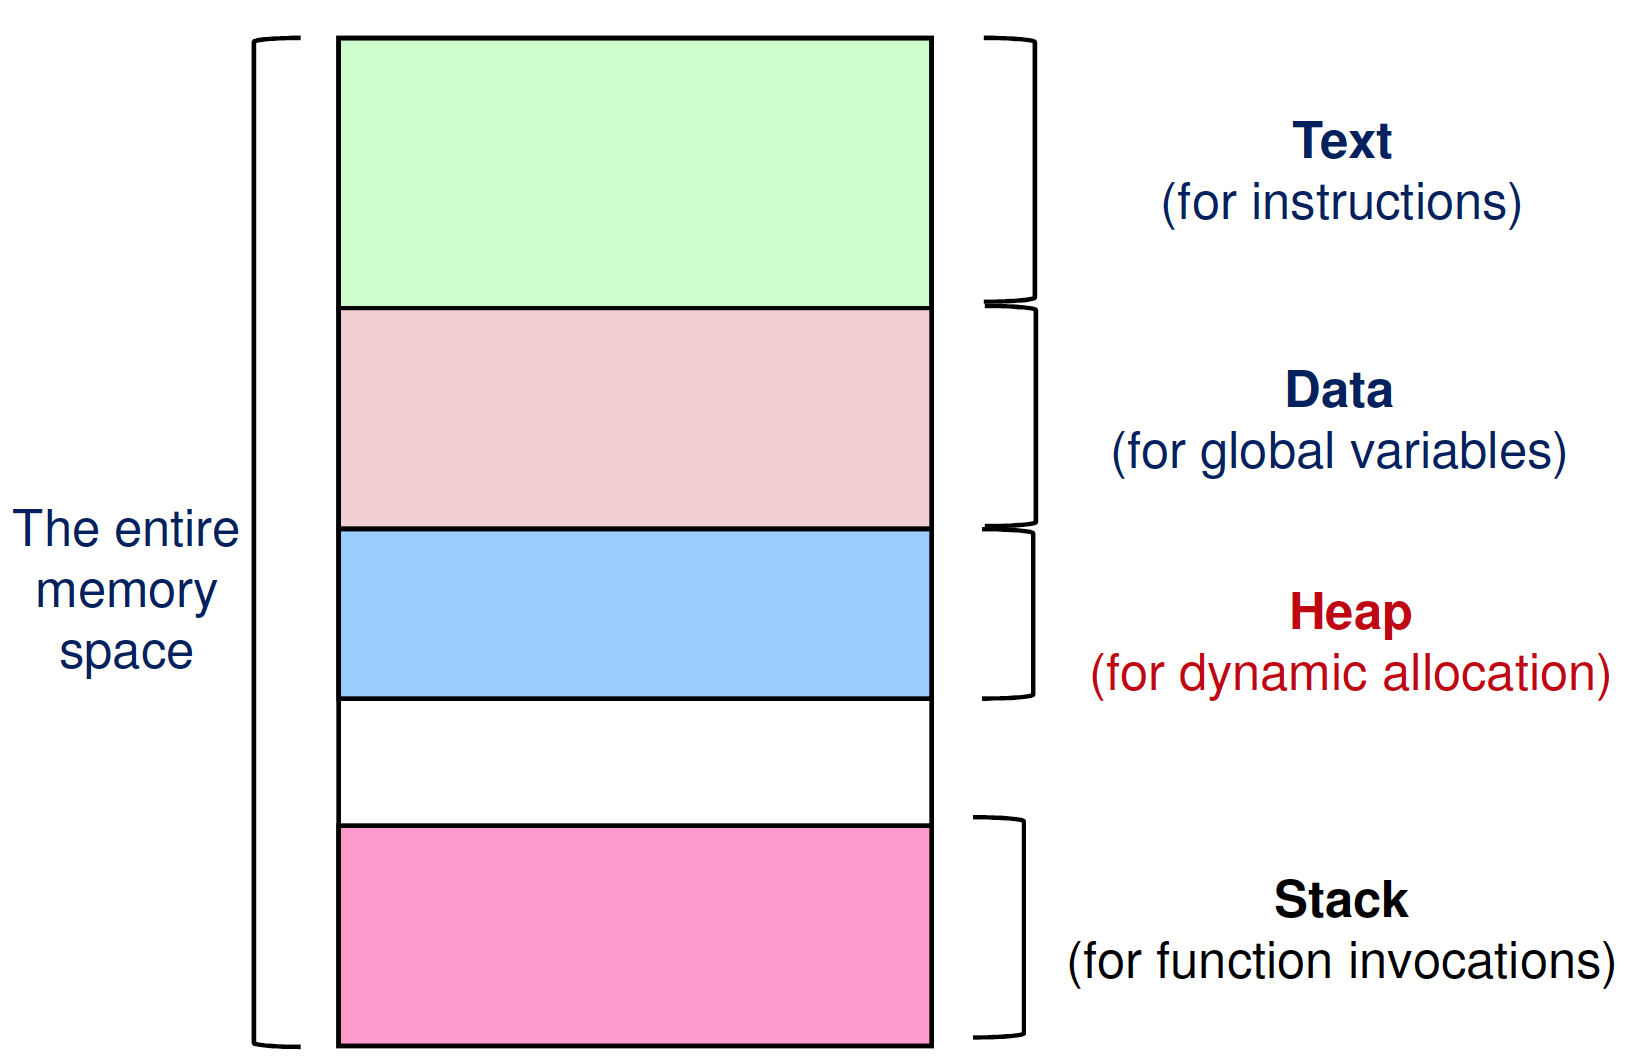
\includegraphics[width=\linewidth]{stack-memory}
  \end{tabularx}
  \begin{tabularx}{0.25\columnwidth}{X}
    Note: \\ in this case, stack grows upwards, heap grows downwards
  \end{tabularx}

  \subsection{Stack Memory}
  \begin{itemize}
    \item New memory region to store information of a function invocation
    \item Described by a \textbf{stack frame}, containing: Return address of the caller (PC, old SP), Arguments for the function, Storage for local variables, Frame Pointer, Saved Registers
    \item \textbf{Stack Pointer} = The top of stack region (first unused location)
    \item \textbf{Frame Pointer} = points to a fixed location in a stack frame
    \item \textbf{Saved Registers} = memory to temporarily hold GPR value during \textbf{register spilling}
  \end{itemize}
  \subsubsection{Function Call Convention}
  E.g. On executing function call, \textbf{Caller}: Pass parameters with registers and/or stack, Save Return PC on stack; \textbf{Callee}: Save the old FP, SP, Allocate space for local vars on stack, adjust SP (Stack Pointer) \\
  On returning from function call, \textbf{Callee}: Restore saved registers, FP, SP; \textbf{Caller}: Continues execution
  \subsection{Dynamically Allocated Memory}
  Using a separate \textbf{heap memory region}
  \subsection{Process Identification \& Process State}
  \begin{itemize}
    \item Using process ID \textbf{(PID)}, a unique number among the processes.
    \item OS dependent: Are PID's reused? Are there reserved PID's? Does it limit max number of processes?
  \end{itemize}
  \begin{tabular}{l}
    \textbf{5 State Process Model}: \\
    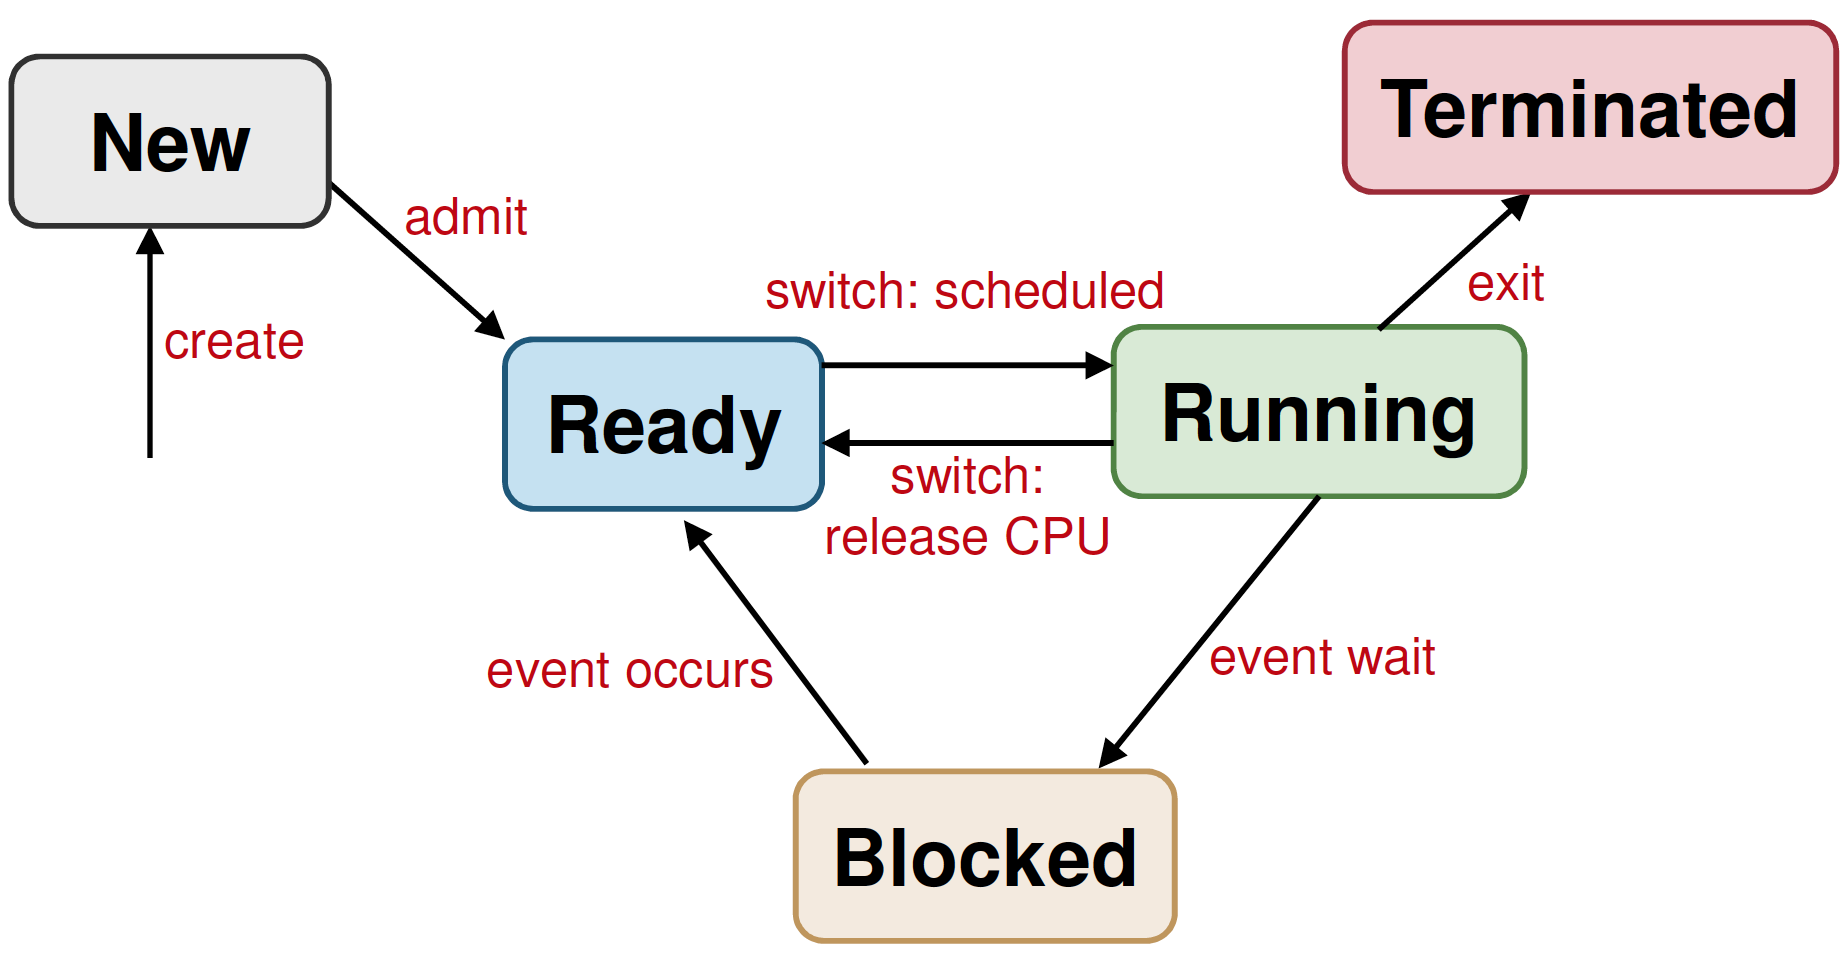
\includegraphics[width=0.55\linewidth]{process-state}
  \end{tabular}
  \begin{tabularx}{0.4\columnwidth}{X}
    \begin{itemize}
      \item \textbf{Process State} = indication of the execution status
    \end{itemize}
  \end{tabularx}
  \begin{enumerate}
    \item \textbf{New}: process created, may still be initialising, not yet ready
    \item \textbf{Ready}: process is waiting to run
    \item \textbf{Running}: process being executed on CPU
    \item \textbf{Blocked}: process waiting, can't execute till event is available
    \item \textbf{Terminated}: process finished execution, may require OS cleanup
  \end{enumerate}
  \textbf{Transitions}:
  \begin{itemize}
    \item nil -> New (Create)
    \item New -> Ready (Admit): Process ready to be scheduled
    \item Ready -> Running (Switch): Process selected to run
    \item Running -> Ready (Switch): Process gives up CPU voluntarily or preempted by scheduler
    \item Running -> Blocked (Event wait): e.g. syscall, waiting for I/O, ...
    \item Blocked -> Ready (Event occurs)
  \end{itemize}
  \subsection{Process Table \& Process Control Block}
  \begin{itemize}
    \item \textbf{PCB/Process Table Entry} = entire execution context for a process
    \item \textbf{Process Table} =  maintains PCB for all processes, stored as one table
    \item Issues: Scalability, Efficiency
  \end{itemize}
  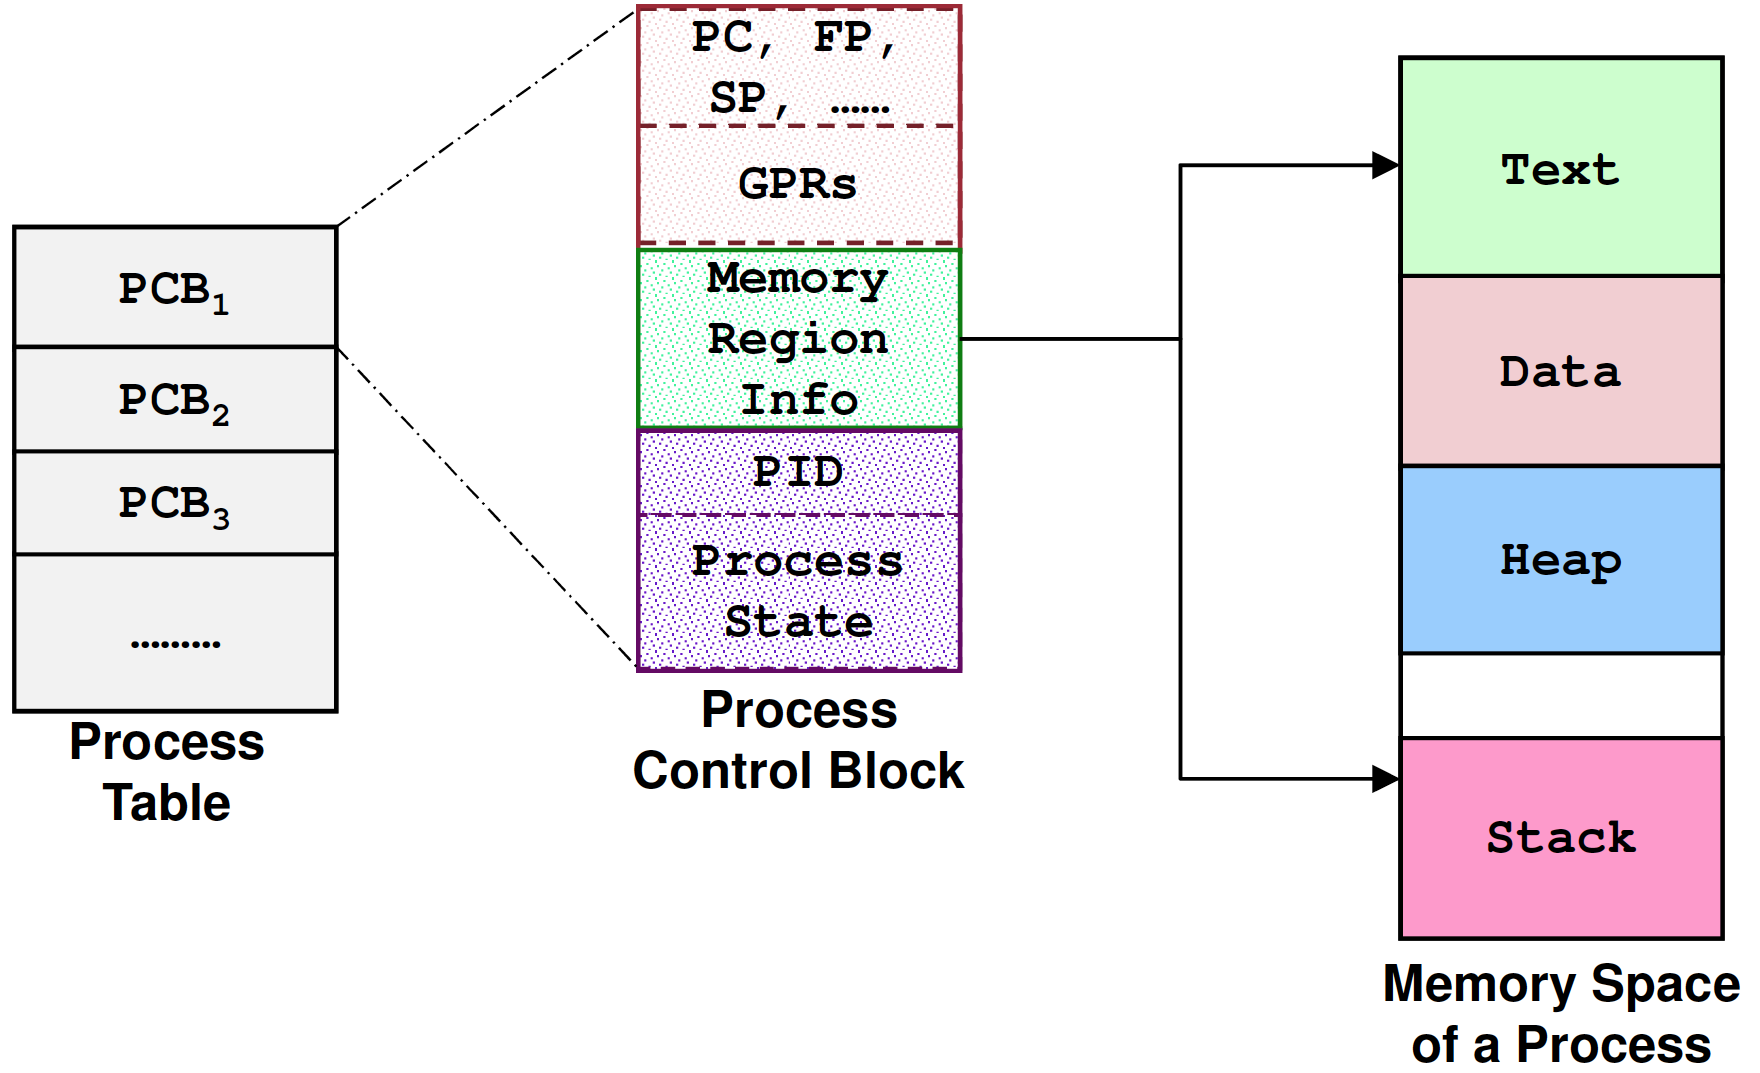
\includegraphics[width=0.7\linewidth]{process-table}
  \subsection{System Calls}
  \begin{itemize}
    \item API to OS -- different from normal function call in that have to change from user mode -> kernel mode
    \item General System Call Mechanism:
          \begin{enumerate}
            \item User program invokes the library call (using normal function call mechanism)
            \item Library call places the system call number in a designated location (e.g. register)
            \item Library call executes a special instruction to switch user -> kernel mode (commonly known as TRAP)
            \item In kernel mode, the dispatching to the appropriate system call handler by dispatcher
            \item System call handler is executed
            \item System call handler ended, control return to library call, switch kernel -> user mode
            \item Library call return to user program via normal function return mechanism
          \end{enumerate}
  \end{itemize}
  \subsection{Exception \& Interrupt}
  \textbf{Exception}:
  \begin{itemize}
    \item Synchronous, occurring due to program execution
    \item Effect: have to execute an \textbf{exception handler}, similar to a forced function call
  \end{itemize}
  \textbf{Interrupt}:
  \begin{itemize}
    \item External events interrupting execution, usually hardware-related
    \item Asynchronous, occurring independent of program execution
    \item Effect: execution is suspended, have to execute \textbf{interrupt handler}
  \end{itemize}
  \subsection{Process Abstraction: Unix}
  \begin{itemize}
    \item \mintinline{C}{int fork();} duplicate current executable, returns PID of newly created process (for parent) or 0 (for child)
    \item \mintinline{C}{int execl(const char *path, const char *arg0, ..., const char *argN, NULL);} replaces current executing process image, does not return unless error. Will not exit on error.
    \item \mintinline{C}{void exit(int status);} \texttt{status} is 0 for normal, else problematic. Does not return.
    \item \mintinline{C}{int wait(int *status);} returns the PID of terminated child, status stores exit status. Blocking.
  \end{itemize}
  \textbf{Zombie process} = (1) parent terminates before child -- \texttt{init} becomes pseudo-parent, who will call \texttt{wait} on children (2) child process terminates but parent did not call \texttt{wait} -- child becomes zombie, can fill up processs table
  \section{Process Scheduling}
  3 categories of \textbf{processing environment}: (1) \textbf{Batch Processing}: no user, no interaction, no need to be responsive, (2) \textbf{Interactive}: with active user interacting, need to be responsive, consistent in response time, (3) \textbf{Real-time Processing}: deadline to meet, usually periodic process
  \subsection{Criteria for Scheduling Algorithms}
  \begin{itemize}
    \item \textbf{Fairness}: fair share of CPU time, no starvation
    \item \textbf{Balance}: all parts of the computing system should be utilised
  \end{itemize}
  \subsection{Types of scheduling policies}
  \begin{itemize}
    \item \textbf{Non-preemptive (cooperative)} -- a process stays scheduled until it blocks/gives up the CPU voluntarily
    \item \textbf{Preemptive}: A process is given a fixed time quota to run (possible to block or yield early), at the end of the time quota, the running process is suspended.
  \end{itemize}
  \subsection{Scheduling a process}
  \begin{enumerate}
    \item Scheduler is triggered (OS takes over)
    \item If context switch is needed: context of current running process is saved, placed on blocked/ready queue
    \item Pick a suitable process \textbf{P} to run based on scheduling algorithm
    \item Setup the context for \textbf{P}
    \item Let process \textbf{P} run
  \end{enumerate}
  \subsection{Scheduling for Batch Processing}
  Criteria:
  \begin{itemize}
    \item \textbf{Turnaround time}: Total time taken
    \item \textbf{Throughput}: Rate of task completion
    \item \textbf{CPU Utilisation}: \% of time when CPU is working on a task
  \end{itemize}
  \subsubsection{First-Come First-Served (FCFS)}
  \begin{itemize}
    \item Tasks are stored on a FIFO queue based on arrival time. Pick the head of queue to run until (task is done OR task is blocked). Blocked task removed from queue, when it is ready again, placed at back of queue like a newly arrived task.
    \item \textbf{Guaranteed} to have no starvation: no of tasks in front of task X in FIFO is always decreasing -> task X will get its chance eventually.
    \item Shortcoming: \textbf{Convoy Effect} -- due to non-preemptiveness, one slow process (CPU intensive) slows down the performance of the entire set of processes.
  \end{itemize}
  \subsubsection{Shortest Job First (SJF)}
  \begin{itemize}
    \item Select the task with the smallest total CPU time, thus \textbf{guaranteeing} smallest average waiting time.
    \item Shortcomings: Need to know total CPU time for a task in advance (have to guess if not available), starvation is possible (biased towards short jobs, long jobs may never get a chance)
    \item Predicting CPU Time, common approach (\textbf{Exponential Average}):\\
          $\text{Predicted}_{n+1} = \alpha \text{Actual}_n + (1-\alpha)\text{Predicted}_n$, where $\alpha =$ degree of weighting decrease, higher $\alpha$ discounts older observations faster
  \end{itemize}
  \subsubsection{Shortest Remaining Time (SRT)}
  \begin{itemize}
    \item Select job with shortest remaining (or expected) time.
    \item Variation of SJF that is preemptive and uses remaining time.
    \item New job with shorter remaining time can preempt currently running job
    \item Provide good service for short jobs even when they arrive late
  \end{itemize}

  \subsection{Scheduling for Interactive Systems}
  \begin{itemize}
    \item
          Criteria:
          \begin{itemize}
            \item \textbf{Response time}: Time between request and response by system
            \item \textbf{Predictability}: Lesser variation in response time
          \end{itemize}
    \item Preemptive scheduling algorithms are used to ensure good response time, thus scheduler needs to run periodically.
    \item \textbf{Timer interrupt} = interrupt that goes off periodically based on hardware clock
    \item Timer interrupt handler \textbf{invokes OS scheduler}.
    \item \textbf{Interval of Timer Interrupt (ITI)} typically 1-10ms
    \item \textbf{Time Quantum} = execution duration given to a process, can be constant/variable, must be multiple of ITI (commonly 5-100ms)
  \end{itemize}
  \subsubsection{Round Robin (RR)}
  \begin{itemize}
    \item Tasks stored in a FIFO queue, pick task from head of queue until (time quantum elapsed OR task gives up CPU voluntarily OR task blocks)
    \item Basically a preemptive version of FCFS
    \item Response time guarantee: given $n$ tasks and quantum $q$, time before a task get CPU is bounded by $(n-1)q$
    \item Choice of time quantum: big = better CPU util, longer waiting time; small = bigger overhead (worse CPU util) but shorter waiting time
  \end{itemize}
  \subsubsection{Priority Scheduling}
  \begin{itemize}
    \item Assign a priority value to all tasks, select task with highest priority value.
    \item Preemptive: highest priority process can preempt running process with lower priority
    \item Non-preemptive: late coming high priority process has to wait for next round of scheduling
    \item \textbf{Shortcomings}: Low priority process can starve, worse in preemptive variant
    \item \textbf{Possible solutions}: Decrease the prioty of currently running process after every time quantum, Given the current running process a time quantum -- this process not considered in the next round of scheduling
    \item Generally hard to guarantee/control exact amount of CPU time given to a process
    \item \textbf{Priority Inversion}: 3 processes, priorities Hi, Mi, Lo. L locks resource, M pre-empts L, A arrives and tries to lock same resource as L. Then M continues executing although H has higher priority.
  \end{itemize}
  \subsubsection{Multi-level Feedback Queue (MLFQ)}
  \begin{itemize}
    \item Adaptive, minimising both response time for IO-bound and turnaround time for CPU-bound
    \item Rules:
          \begin{itemize}
            \item Priority(A) $>$ Priority(B) -> A runs
            \item Priority(A) == Priority(B) -> A and B in RR
            \item New job -> highest priority
            \item If a job fully utilised its time slice -> priority reduced
            \item If a job gives up/blocks before it finishes the time slice -> priority retained
          \end{itemize}
    \item \textbf{Shortcomings}: (1) Starvation -- if there are too many interactive jobs, long-running jobs will starve, (2) gaming the scheduler by running for 99\% of time quantum, then relinquish the CPU, (3) a program may change its behaviour CPU-bound -> interactive
    \item Possible solution:
          \begin{itemize}
            \item \textbf{Priority boost}: after some time period S, move all jobs to the highest priority. Guaranteeing no starvation as highest priority -> RR, and the case when CPU-bound job has become interactive
            \item \textbf{Better accounting}: Once a job uses up its time allotment at a given level, its priority is reduced
          \end{itemize}
  \end{itemize}
  \subsubsection{Lottery Scheduling}
  \begin{itemize}
    \item Give out "lottery tickets" to processes. When a scheduling decision is needed, a ticket is chosen randomly among eligible tickets.
    \item In the long run, a process holding X\% of tickets can win X\% of the lottery held and use the resource X\% of the time.
    \item Reponsive: newly created process can participate in next lottery
    \item Good level of control: A process can be given lottery tickets to be distributed to its child process, an important process can be given more lottery tickets, each resource can have its own set of tickets (different proportion of usage per resource per task)
    \item Simple implementation
  \end{itemize}

  \section{Process Alternative -- Threads}
  \begin{itemize}
    \item Motivation:
          \begin{itemize}
            \item Process is expensive: under \texttt{fork()} model -- duplicate memory space and process context, context switch requires saving/restoration of process information
            \item Hard for independent processes to communicate with each other: independent memory space -- no easy way to pass information, requires Inter-Process Communication (IPC)
          \end{itemize}
    \item A traditional process has a single thread of control -- only one instruction of the whole program is executing at any one time. Instead, we add more threads of control such that multiple parts of the program are executing simultaneously conceptually.
  \end{itemize}
  \subsection{Process and Thread}
  \begin{itemize}
    \item A single process can have multiple threads
    \item Threads in the same process shares: \textbf{Memory Context} (text, data, heap), and \textbf{OS Context} (PID, other resources like files, etc.)
    \item Unique information needed for each thread: Identification (usually thread id), Registers (general purpose \& special), "stack"
    \item Process context switch involves: OS Context, Hardware Context, Memory Context
    \item Thread switch within the same process involves: Hardware context (registers, "stack" -- actually just changing FP and SP)
  \end{itemize}
  \subsection{Benefits}
  \begin{itemize}
    \item \textbf{Economy}: requires much less resources
    \item \textbf{Resource sharing}: no need for additional information passing mechanism
    \item \textbf{Responsiveness}: multithreaded programs can appear much more responsive
    \item \textbf{Scalability}: Multithreaded program can take advantage of multiple CPU's
  \end{itemize}
  \subsection{Problems}
  \begin{itemize}
    \item \textbf{System call concurrency} -- have to guarantee correctness and determine the correct behaviour
    \item \textbf{Process behaviour} -- impact on process operations, e.g. does \texttt{fork()} duplicate threads? If single thread executes \texttt{exit()}, hwo abut the whole process, etc.
  \end{itemize}
  \subsection{Thread Models}
  \begin{itemize}
    \item \textbf{User Thread}
          \begin{itemize}
            \item Implemented as a user library, a runtime system in the process handles thread operations
            \item Kernel is not aware of threads in the process.
            \item \textbf{Advantages}: Multithreaded program on ANY OS, thread operations are just library calls, more conigurable and flexible (such as customised thread scheduling policy)
            \item \textbf{Disadvantages}: OS is not aware of threads, scheduling is performed at process level. One thread blocked -> process blocked -> all threads blocked, cannot exploit multiple CPUs
          \end{itemize}
    \item \textbf{Kernel Thread}
          \begin{itemize}
            \item Implemented in the OS, thread operation as system calls.
            \item Thread-level scheduling is possible
            \item Kernel may make use of threads for its own execution
            \item \textbf{Advantages}: Kernel can schedule on thread level
            \item \textbf{Disadvantages}: Thread operation is a syscall (slower and more resource intensive), generally less flexible (used by all multithreaded programs -- many features: expensive, overkill for simple program, few features: not flexible enough for some)
          \end{itemize}
    \item \textbf{Hybrid Thread Model}:
          \begin{itemize}
            \item Have both kernel and user threads, OS schedule on kernel threads only, user thread can bind to a kernel thread.
            \item Great flexibility (can limit concurrency of any process/user)
          \end{itemize}
  \end{itemize}
  \subsection{Threads on Modern Processor (Intel Hyperthreading)}
  \begin{itemize}
    \item Threads started off as software mechanism: Userspace lib -> OS aware mechanism
    \item Hardware support on modern processors, supplying multiple sets of registers to allow threads to run natively and parallelly on the same core: \textbf{Simultaneous Multi-Threading (SMT)}
  \end{itemize}
  \subsection{POSIX Threads: \texttt{pthread}}
  \begin{itemize}
    \item Standard by IEEE, defining API and behaviour.
    \item \mintinline{C}{int pthread_create(pthread_t* tidCreated, const pthread_attr_t* threadAttributes, void* (*startRoutine) (void*), void* argForStartRoutine);}
    \item \mintinline{C}{int pthread_exit(void* exitValue)}
    \item \mintinline{C}{int pthread_join(pthread_t threadID, void **status);}
    \item except for \texttt{pthread\_exit}, return 0 = success
  \end{itemize}

  \section{Inter-Process Communication}
  \begin{itemize}
    \item 2 common IPC mechanisms: Shared-Memory \& Message Passing
    \item 2 Unix-specific IPC mechanisms: Pipe and Signal
  \end{itemize}
  \subsection{Shared-Memory}
  \begin{itemize}
    \item General idea: Process $p_1$ creates a shared memory region $M$, process $p_2$ attaches $m$ to its own memory space. $p_1$ and $p_2$ can now commmunicate suing memory region $M$
    \item OS involved only in creating and attaching shared memory region
    \item \textbf{Advantages}: Efficient (only initial steps involves OS), Ease of use (information of any type or size can be written easily)
    \item \textbf{Disadvantages}: Synchronisation (shared resource -> need to synchronise access), Implementation is usually harder
    \item In Unix: (1) create/locate shared memory region $M$, (2) Attach $M$ to process memory space, (3) Read/Write $M$, (4) Detach $M$ from memory space after use, (5) Destroy $M$ (only 1 process, can only destroy if $M$ is not attached)
  \end{itemize}
  \subsection{Message Passing}
  \begin{itemize}
    \item General idea: process $p_1$ prepares a message $M$ and send it to process $p_2$, $p_2$ receives the message $M$
    \item Message has to be stored in kernel memory space, every send/receive operation is a syscall
    \item \textbf{Advantages}: Portable (can be easily implemented on different processing environment), Easier synchronisation (using synchronous primitive)
    \item \textbf{Disadvantages}: Inefficient (usually requiring OS intervention), Harder to use (message usually limited in size and/or format)
  \end{itemize}
  \subsubsection{Naming \textmd{(how to identify the other party in the comm):}}
  \begin{itemize}
    \item \textbf{Direct Communication}
          \begin{itemize}
            \item Sender/receiver explicitly name the other party
            \item Characteristics: 1 link/pair of communicating processes, need to know the identity of the other party
          \end{itemize}
    \item \textbf{Indirect Communication}
          \begin{itemize}
            \item Message are sent to/received from message storage (known as mailbox or port)
            \item Characteristic: 1 mailbox can be shared among a number of processes
          \end{itemize}
  \end{itemize}
  \subsubsection{Synchronisation \textmd{(behaviour of the sending/receiving ops)}}
  \begin{itemize}
    \item \textbf{Blocking primitives} (synchronous): sender/receiver is blocked until message is received/has arrived
    \item \textbf{Non-blocking Primitive} (asynchronous): sender resume operation immediately, receiver either receive message if available or some indication that message is not ready yet.
  \end{itemize}
  \subsection{Unix Pipes}
  \begin{itemize}
    \item A communication channel with 2 ends, for reading and writing.
    \item A pipe can be shared between 2 processes (producer-consumer)
    \item Behaviour: like an anonymous file, FIFO (in-order access)
    \item Pipe functions as \textbf{circular bounded byte buffer with implicit synchronisation}: writers wait when buffer full, readers wait when buffer empty
    \item Variants: Multiple readers/writers, half-duplex (unidirectional) or full-duplex (bidirectional)
    \item \mintinline{C}{int pipe(int fd[]);} returns 0 = success. \mintinline{C}{fd[0]} reading end, \mintinline{C}{fd[1]} writing end
  \end{itemize}
  \subsection{Unix Signal}
  \begin{itemize}
    \item An async notification regarding an event sent to a process/thread
    \item Recipient of signal handle by a default set of handlers OR user-supplied handler
    \item Common signals in Unix: SIGKILL, SIGSTOP, SIGCONT, etc.
  \end{itemize}

  \section{Synchronization}
  \subsection{Race Condition}
  \begin{itemize}
    \item When 2/more processes execute concurrently in interleaving fashion AND share a modifiable resource resulting in non-deterministic execution.
    \item Solution: designate code segment with race condition as \textbf{critical section} where at any point in time only 1 process can execute.
  \end{itemize}
  \subsection{Critical Section}
  Properties of correct implementation:
  \begin{itemize}
    \item \textbf{Mutual Exclusion}: if a process is executing in critical section, all other processes are prevented from entering it
    \item \textbf{Progress}: If no process is in critical section, one of the waiting processes should be granted access
    \item \textbf{Bounded Wait}: After a process $p_i$ requests to enter the critical section, $\exists$ an upper-bound of number of times other processes can enter the critical section before $p_i$
    \item \textbf{Independence}: process not executing in critical section should never block other processes
  \end{itemize}
  Symptoms of incorrect synchronisation:
  \begin{itemize}
    \item \textbf{Deadlock}: all processes blocked -> no progress
    \item \textbf{Livelock}: processes keep changing state to avoid deadlock and make no other progress, typically processes are not blocked
    \item \textbf{Starvation}: some processes are blocked forever
  \end{itemize}
  \subsection{Implementations of Critical Section}
  \subsubsection{Test-and-set: an atomic instruction}
  \begin{itemize}
    \item Load the current content at \texttt{MemoryLocation} into \texttt{Register}, Stores a \texttt{1} into \texttt{MemoryLocation}
    \item Disadvantage: busy waiting -- wasteful use of processing power
  \end{itemize}
  \subsubsection{Peterson's Algorithms}
  \begin{minted}{C}
bool flag[2] = {false, false};
int turn;
  \end{minted}
  \begin{multicols*}{2}
    \begin{minted}{C}
flag[0] = true;
turn = 1;
while (flag[1] && turn == 1) {
  // busy wait
}
// critical section
flag[0] = false;
    \end{minted}
    \begin{minted}{C}
flag[1] = true;
turn = 0;
while (flag[1] && turn == 0) {
  // busy wait
}
// critical section
flag[1] = false;
    \end{minted}
  \end{multicols*}
  Disadvantages:
  \begin{itemize}
    \item \textbf{Busy Waiting}, wasteful use of processing power
    \item \textbf{Low level}: higher-level programming construct desirable to simplify mutex and less error prone
    \item \textbf{Not general}: general synchronisation mechanism is desirable, not just mutex
  \end{itemize}
  \subsubsection{Semaphore}
  A generalised synchronisation mechanism, providing a way to block a number of processes and a way to unblock one/more sleeping process(es)
  \begin{itemize}
    \item \texttt{wait(S)}: if $S$ is (+)-ve, decrement. If $S$ is now (-)ve, go to sleep
    \item \texttt{signal(S)}: increment S, if pre-increment $S$ negative, wakes up 1 sleeping process
  \end{itemize}
  \textbf{Properties}
  \begin{itemize}
    \item Given $S_\text{initial} \geq 0$, where \#signal(S) = no of \texttt{signal()} executed, \#wait(S) = no of \texttt{wait()} completed
    \item \textbf{Invariant}: $S_\text{current} = S_\text{initial} +$ \#signal(S) $- $ \#wait(S)
  \end{itemize}
  Binary semaphore, $S = 0$ or $1$ known as mutex (mutual exclusion)\\
  Deadlock still possible
  \subsection{Classical Synchronisation Problems}
  \begin{itemize}
    \item \textbf{Producer-Consumer}: produce only if buffer not full, consume only if buffer not empty
    \item \textbf{Reader-Writers}: writer exclusive access, reader can share
    \item \textbf{Dining Philosophers}: assign partial order to the resources, establishing convention that all resources will be requested in order. E.g. label forks 1-5, and always pick up lower-numbered fork first.
  \end{itemize}
  \subsection{Synchronisation Implementations}
  \begin{itemize}
    \item POSIX semaphores
    \item pthread\_mutex\_t: \texttt{pthread\_mutex\_lock}, \texttt{pthread\_mutex\_unlock}
    \item pthread\_cond\_t: \texttt{pthread\_cond\_wait}, \texttt{pthread\_cond\_signal}, \texttt{pthread\_cond\_broadcast}
  \end{itemize}

  \section{Memory Management}
  \begin{itemize}
    \item \textbf{Logical address}: how the process views its memory space
    \item \textbf{Base register}: start offset
    \item \textbf{Limit register}: range of memory space of current process
  \end{itemize}

  \subsection{Contiguous Memory Management}
  \begin{itemize}
    \item 2 schemes of allocating memory partition:
          \begin{itemize}
            \item \textbf{Fixed-size}\\
                  \textbf{Pros}: Easy to manage, fast to allocate (all free partitions are the same, no need to choose), \textbf{Cons}: partition size need to be large enough to contain the largest process (internal fragmentation)
            \item \textbf{Variable-size}\\
                  \textbf{Pros}: Flexible, removes internal fragmentation, \textbf{Cons:} Need to maintain more information in OS, takes more time to locate appropriate region, external fragmentation
          \end{itemize}
    \item \textbf{Merging and Compaction}: consolidate holes (time-consuming)
    \item \textbf{Allocation algo}: \textbf{First-Fit}: first large enough hole, \textbf{Best-Fit}: smallest large enough hole, \textbf{Worst-Fit}: largest hole
  \end{itemize}
  \subsubsection{Allocation Algo: Buddy System}
  \begin{itemize}
    \item Provides efficient: (1) Partition splitting, (2) locating good match of free partition, (3) Partition de-allocation and coalescing
    \item Free block is split into half repeatedly to meet request, two halves form buddy blocks. When buddy blocks are both free, merge.
    \item Keep array \texttt{A[0..K]} where $2^K = $ largest allocatable block size.
    \item \texttt{A[J]} is a linked list, keeps tracks of free block(s) of size $2^J$
    \item Blocks $B$ and $C$ are buddy of size $S$, if the $S$th bit of B and C are complements (0 and 1) and the leading bits up to the $S$th bit are the same (e.g. 10100 and 10000)
    \item Allocating a block of size $N$:
  \end{itemize}
  \begin{minted}{Ruby}
S = Math.log2(N).ceil # smallest S s.t. 2^S <= N
while true
  # If got free block, remove from list and allocate
  allocate(A[S].shift) and return if A[S].size > 0
  # Else, find smallest R s.t. A[R] has a free block
  # repeatedly split s.t. A[S..R-1] has a new free block
  R = (S+1).upto(K).find { |i| A[i].size > 0 }
  (R+1).downto(S).each{ |i| split A[i], from: A[i+1] }
end
\end{minted}
  \begin{itemize}
    \item To free a block $B$:
  \end{itemize}
  \begin{minted}{Ruby}
def free(B)
  S = Math.log2(B.size).ceil
  C = A[S].find_free_buddy_of(B)
  A[S].append(B) and return if C.nil? # buddy not free
  A[S].delete(C)
  B2 = merge(B, C) # merge buddies
  free(B2)
end
\end{minted}

  \section{Disjoint Memory Schemes}
  \subsection{Paging Scheme}
  \begin{itemize}
    \item Physical mem is split into fixed-size regions: \textbf{Physical Frame}
    \item Logical mem of a process is split into regions of the same size: \textbf{Logical Page}
    \item Logical memory space is contiguous but occupied physical memory region can be disjointed.
    \item Paging removes external but \textbf{not internal} fragmentation.
  \end{itemize}
  \subsubsection{Logical Address Translation}
  \begin{itemize}
    \item \textbf{Page Table}: lookup table for logical address translation (logical page <-> physical frame). Need to know 2 things: $F = $ physical frame number, Offset = from start of physical frame
    \item Physical address = $F \times$ physical frame size $+$ Offset
    \item Given: frame size = $2^n$, $m$ bits of logical address

  \end{itemize}
  \begin{tabularx}{0.5\columnwidth}{X}
    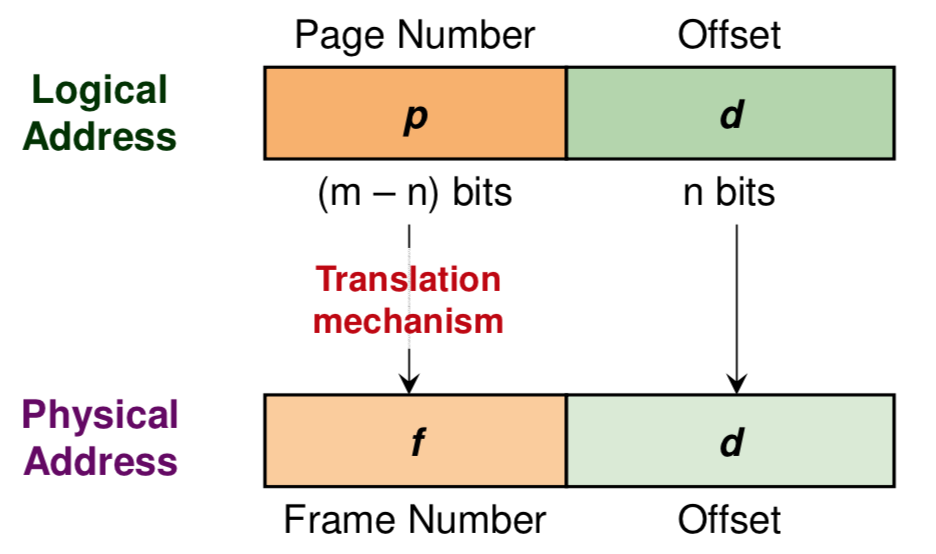
\includegraphics[width=\linewidth]{translation}
  \end{tabularx}
  \begin{tabularx}{0.5\columnwidth}{X}
    \textbf{Logical Address} $LA$: \\$p$ = most significant $m-n$ bits of $LA$,\\
    $d$ = remaining $n$ bits of $LA$
      \\ \\
      \textbf{Physical Address}    \\$PA = f \times 2^n + d$
  \end{tabularx}
  \subsubsection{Implementation}
  \begin{itemize}
    \item \textbf{Pure-software}: OS stores page table information in the PCB\\
          \textbf{Issues}: require 2 mem access for every mem ref (1) read indexed page table entry to get frame number, (2) access actual mem item
    \item \textbf{Hardware support}: Translation Look-aside Buffer (TLB) = cache of a few page table entries
          \begin{itemize}
            \item Use page number to search TLB, either TLB-Hit or TLB-Miss
            \item TLB is part of hardware context. Thus, context switch -> TLB entries are flushed
          \end{itemize}
  \end{itemize}
  \begin{enumerate}
    \item \textbf{(HW)} LA is decomposed into \texttt{<Page\#, Offset>}
    \item \textbf{(HW)} Search TLB for \texttt{Page\#}:
          \begin{enumerate}
            \item TLB-Hit: Use \texttt{<Frame\#, Offset>} to access physical mem. Done.
            \item TLB-Miss: Trap to OS (TLB Fault)
          \end{enumerate}
    \item \textbf{(OS - TLB Fault)} Access full table of the process (in PCB), \texttt{<Page\#>} is the index:
          \begin{enumerate}
            \item If memory resident, replace a TLB entry, return from trap, retry step 1
            \item If non-memory-resident, trap to OS (Page Fault)
          \end{enumerate}
    \item \textbf{(OS - Page Fault)} Locate the page in secondary swap pages. Load the page into a physical frame (applying replacement algo if needed). Update PTE, return from trap, retry step 3
  \end{enumerate}
  \subsubsection{Protection}
  \begin{itemize}
    \item \textbf{Access Right Bits}: each page table entries has several bits to indicate rwx, mem access is checked against the access right bits
    \item \textbf{Valid bit}: each page table entries has a bit to indicate if the page is valid for the process to access. OOB access caught by OS
  \end{itemize}
  \subsubsection{Page sharing}
  Deduplication. Possible usage:
  \begin{itemize}
    \item \textbf{Shared code page}: used by many processes, e.g. C stdlib, syscalls
    \item \textbf{Implement CoW}: upon forking, before any mem value mutation
  \end{itemize}
  \subsection{Segmentation Scheme}
  \begin{itemize}
    \item Some regions may grow/shrink at exec time. Thus putting them in non-contiguous mem space to allow them to grow/shrink freely and easier check whether access is in-range.
    \item Mem space of a process separated into different segments: user code, global vars, heap, stack, lib code, etc.
    \item Logical mem space of a process is a collection of segments
    \item Each segment: has a name and a limit
    \item All mem ref is \texttt{Segment Name + Offset} (e.g. Heap + 245)
    \item Each segment mapped to a contiguous physical mem region (base address + limit)
    \item \textbf{segment id} =  single number representing segment name
    \item Logical address: \texttt{<SegID, Offset>} (\texttt{SegID} used to look up \texttt{<Base, Limit>} in a segment table)
    \item $PA =$ Base + Offset, Offset $<$ Limit for valid access
    \item \textbf{Pros}: Each segment is an independent contiguous mem space (can grow/shrink, protected/shared independently)
    \item \textbf{Cons}: Requires variable-size contiguous memory regions, external fragmentation
  \end{itemize}
  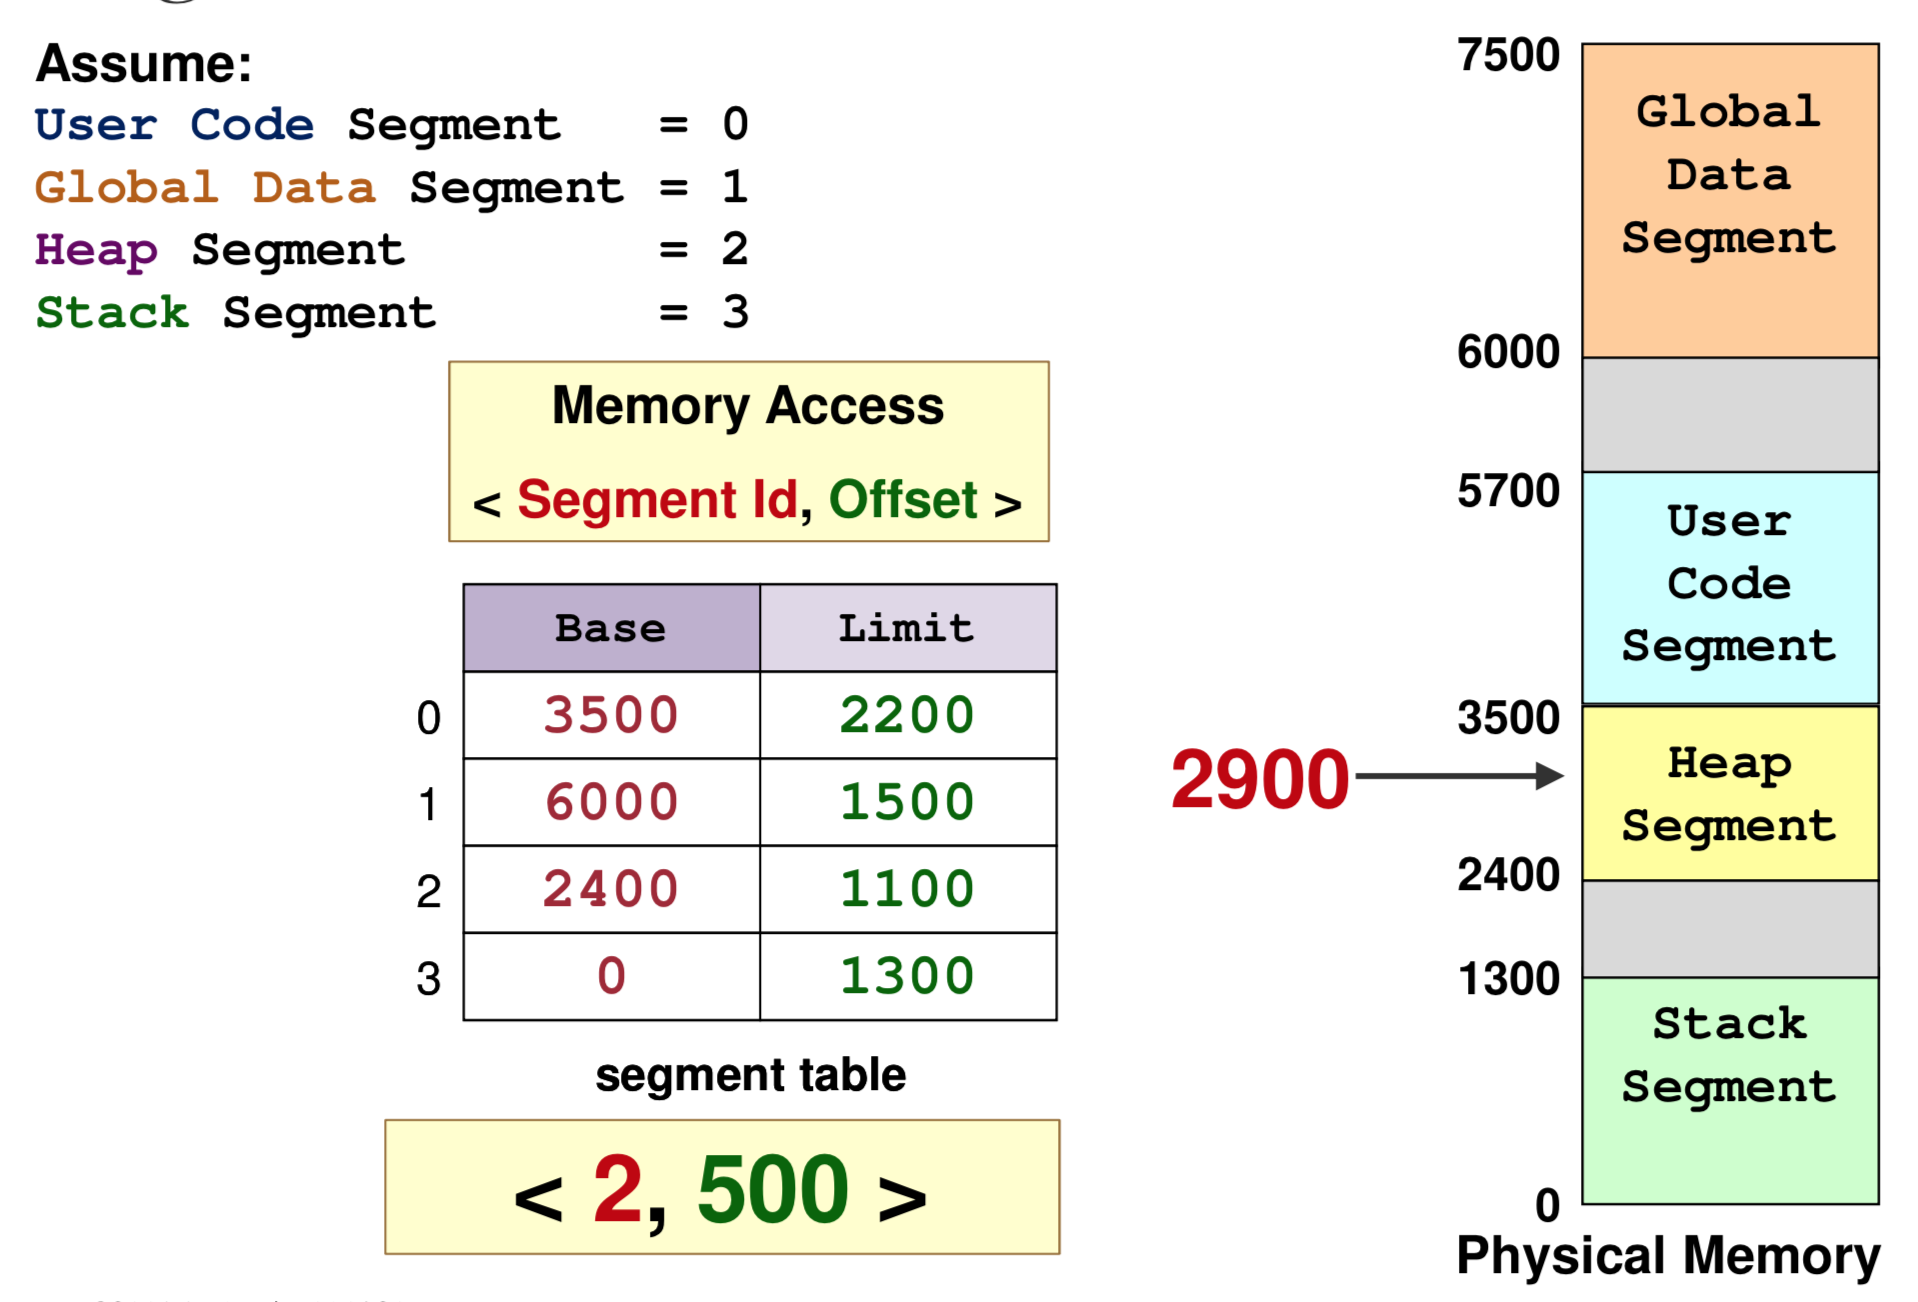
\includegraphics[width=\linewidth]{segmentation}
  \subsection{Segmentation: Hardware Support and combined with Paging}
  Each segment is now composed of several pages instead of a contiguous memory region (each segment has a page table)

  Table: (Segment\#, Page Limit, Page Table Base)

  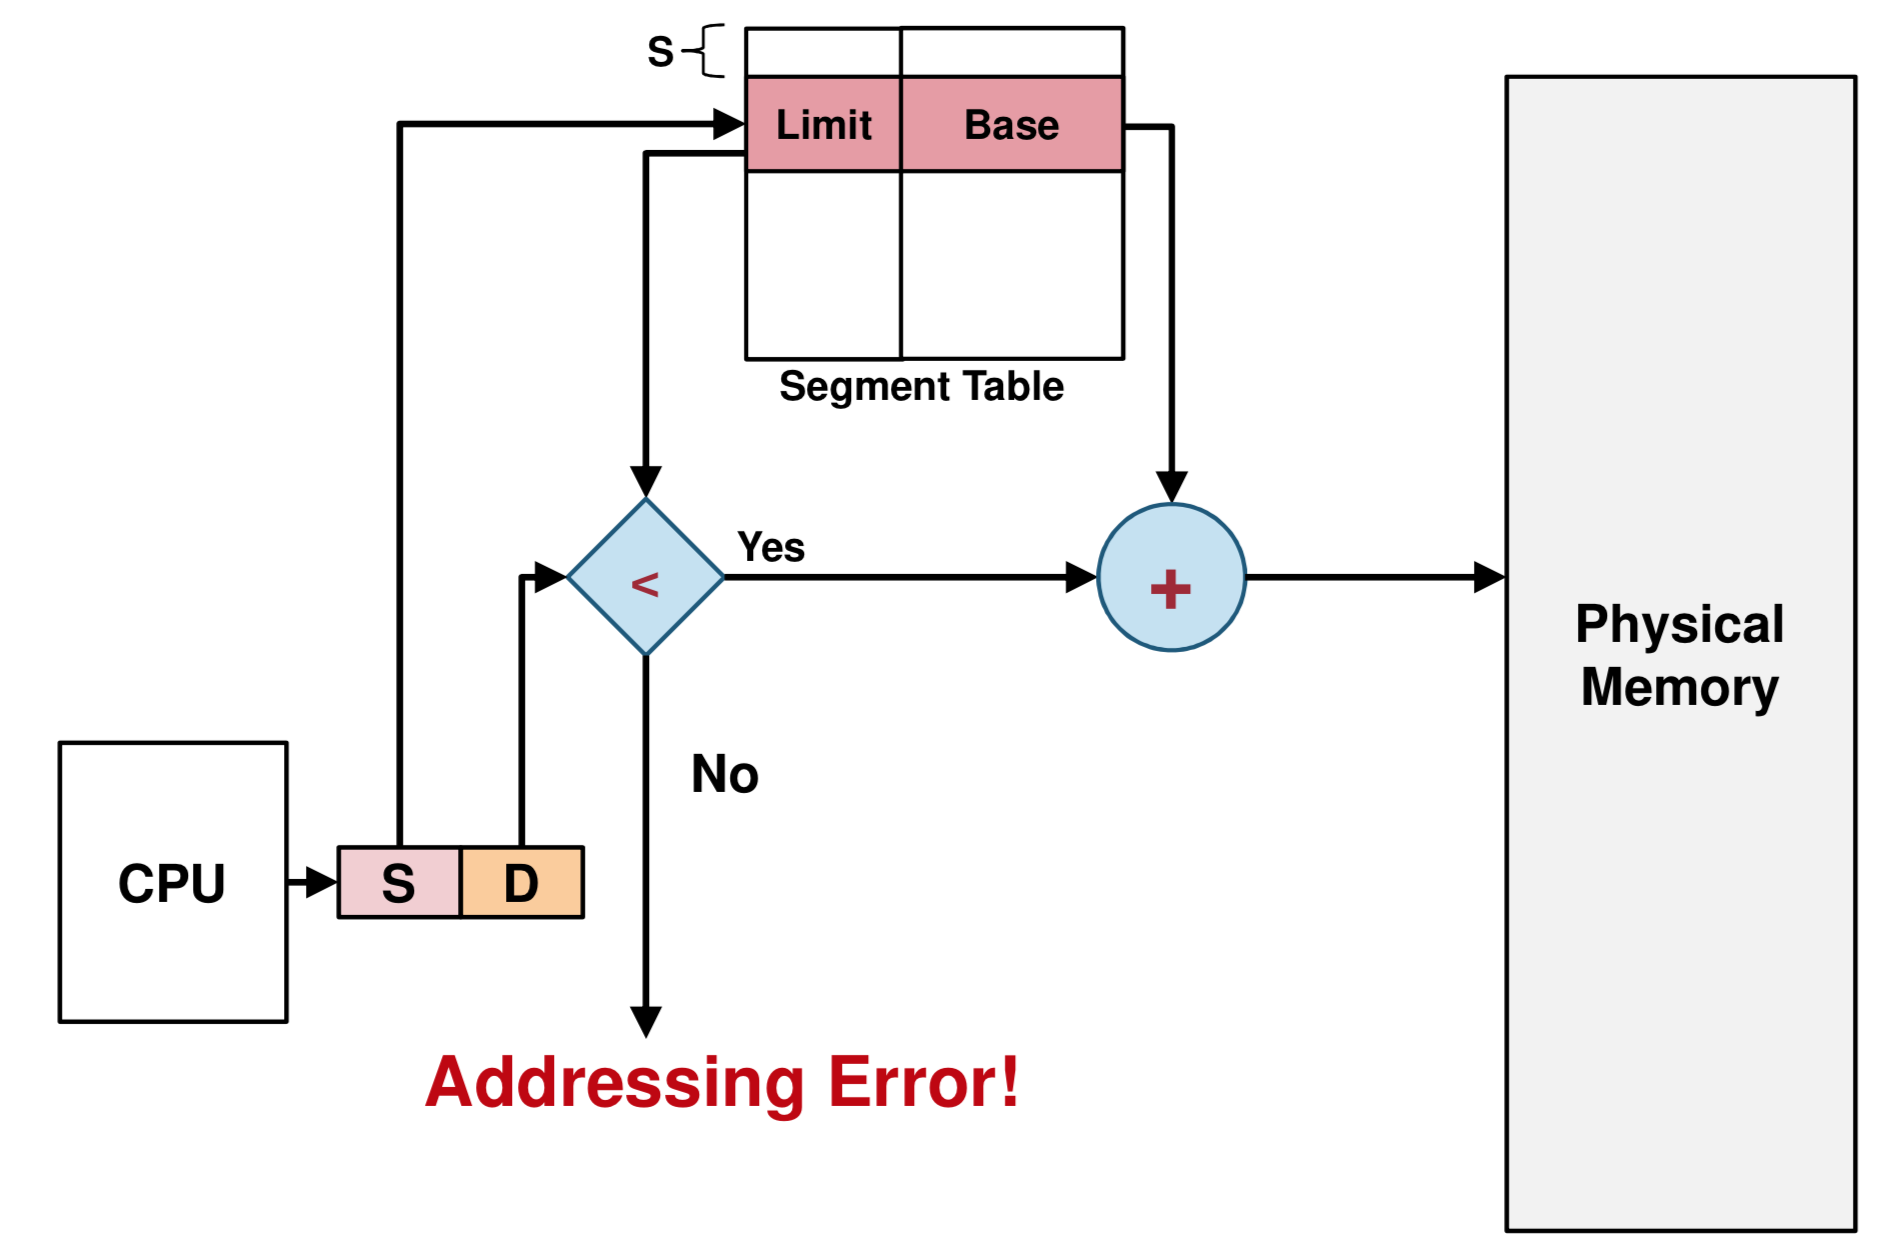
\includegraphics[width=0.8\linewidth]{s}

  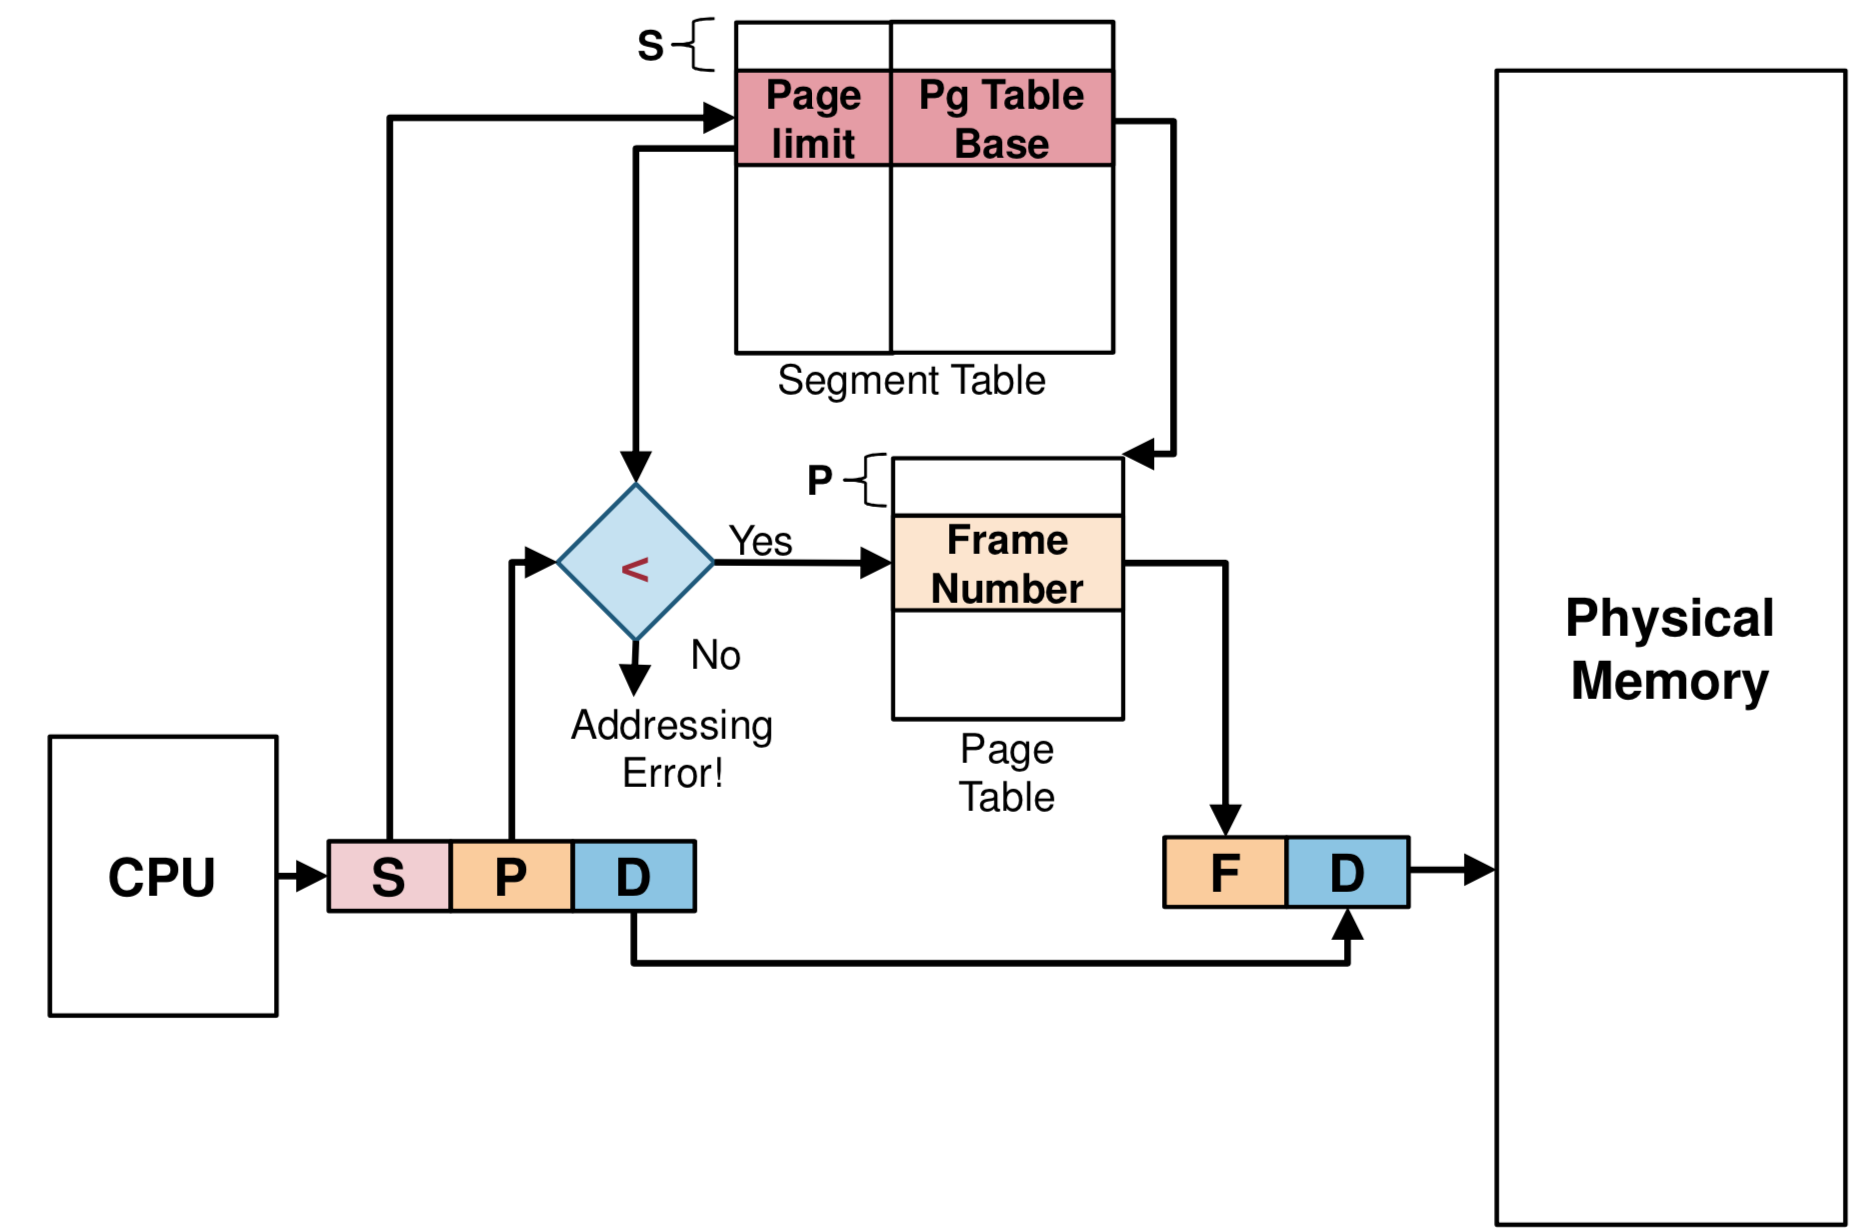
\includegraphics[width=0.8\linewidth]{swp}

  \section{Virtual Memory Management}
  \begin{itemize}
    \item Use page table to translate \textbf{virtual} -> physical address
    \item Extend paging scheme: Some pages may be in physical memory, others in secondary storage.
    \item Use a \texttt{memory\_resident?} bit to distinguish between 2 page-types: \textbf{memory-resident} and \textbf{non-memory-resident}
    \item CPU can only access memory-resident pages. \textbf{Page Fault} (PF) when CPU tries to access non-memory-resident page. OS needs to bring them into physical memory.
    \item Just like cache, exploit \textbf{Temporal} \& \textbf{Spatial} Locality
    \item Accessing page X:
          \begin{enumerate}
            \item If page X \textbf{memory resident}: Access physical mem. Done.
            \item Else \textbf{PF}: Trap to OS
            \item Locate page X in secondary storage
            \item Load page X into a physical memory frame
            \item Update page table
            \item Go to step 1
          \end{enumerate}
  \end{itemize}
  \subsection{Page Table Structure}
  \subsubsection{Direct Paging}
  \begin{itemize}
    \item Keep all entries in a single table
    \item With $2^p$ pages in logical mem space, $p$ bits to specify one unique page, $2^p$ PTE (each containing physical frame number + additional info bits), e.g. Virtual Address: 32 bits, page size = 4 KB, $p = 32 - 12 = 20$, size of PTE = 2 B, PT Size = $2^{20}\times 2$ bytes = 2MB
  \end{itemize}
  \subsubsection{2-Level Paging}
  \begin{itemize}
    \item Split page table into smaller page tables, each with a \textbf{PT number}
    \item Total $2^P$ entries, with $2^M$ smaller PTs, $M$ bits to identify 1 PT, each smaller PT contains $2^{(P-M)}$ entries
    \item Use \textbf{page directory} to keep track, containing $2^M$ indices. Ideally, size of page dir = page size
    \item \textbf{Advantages}: corresponding PT to empty entries in page dir need not be allocated
  \end{itemize}
  \subsubsection{Inverted Page Table}
  \begin{itemize}
    \item Instead of keeping per-process PT, only a \textbf{single} mapping of physical frame to \texttt{<pid, page\#>} (ordered by frame\# instead of page\#)
    \item \textbf{Advantage}: Memory saving, 1 table for all processes
    \item \textbf{Disadvantage}: Slow translation ($O(n)$ to look up a page\#)
  \end{itemize}
  \subsection{Page Replacement Algorithms}
  \begin{itemize}
    \item When a page is evicted: \textbf{clean page} (not modified), \textbf{dirty page} (modified, must write back)
    \item Memory access time: $T_{access} = (1-p)\times T_{mem}+p\times T_{page\_fault}$ where $p$ = prob of PF, $T_{mem}$ = access time for mem-resident page, $T_{page\_fault}$ = access time if PF occurs
    \item Since $T_{page\_fault} >> T_{mem}$, need to reduce $p$ to keep $T_{access}$ reasonable (reduce total no of PF)
  \end{itemize}
  \subsubsection{Optimal Page Replacement (OPT)}
  \begin{itemize}
    \item Replace the page that will not be used again for the longest period of time. Guarantees min no of PF
    \item However, not realisable, need \textbf{future knowledge} of mem refs
    \item Base comparison for other algorithms
  \end{itemize}
  \subsubsection{FIFO}
  \begin{itemize}
    \item Mem pages are evicted based on their loading time
    \item Implementation: OS maintain a queue of resident page numbers. Remove the first page in queue if replacement is needed. Update the queue during PF trap.
    \item \textbf{Advantage}: simple to implement (no HW support needed)
    \item \textbf{Problems}: Belady's Anomaly (more frames, more PF) because FIFO does not exploit temporal locality
  \end{itemize}
  \subsubsection{Least Recently Used (LRU)}
  \begin{itemize}
    \item Make use of temporal locality. Does not suffer from Belady's Anomaly
    \item \textbf{Impl 1}: A logical time counter, incremented for every mem ref. PTE has a time of use field, replace page with smallest time of use.
    \item However, need to search through all pages, and counter is forever increasing (overflow)
    \item \textbf{Impl 2}: Use a stack. If page X is referenced, remove from stack, push on top of stack. Replace the page at bottom of stack.
    \item However, not a pure stack. Entries can be removed from anywhere in the stack. Hard to implement in hardware.
  \end{itemize}
  \subsubsection{Second-Chance Page Replacement (CLOCK)}
  \begin{itemize}
    \item Modified FIFO to give a second chance to pages that are accessed.
    \item Each PTE maintains a reference bit: \textbf{1} = accessed, \textbf{0} = not accessed
    \item Algo:
          \begin{enumerate}
            \item Select oldest FIFO page.
            \item If ref\_bit == 0, page is replaced.
            \item If ref\_bit == 1, page is given 2nd chance: ref\_bit cleared to 0. Arrival time reset (as if newly loaded). Next FIFO page is selected, go to step 2
          \end{enumerate}
    \item Impl: use a \textbf{circular queue} to maintain the pages, with a pointer to the oldest page. To find a page to be replaced, advance until a page with ref\_bit == 0, and clear reference bit as pointer passes.
    \item When all ref\_bit == 1, degenerate into FIFO
  \end{itemize}
  \subsection{Frame Allocation}
  \begin{itemize}
    \item $N$ physical mem frames, $M$ processes competing for frames.
    \item \textbf{Equal allocation} (each process gets $\frac{N}{M}$ frames), \textbf{Proportional Allocation} (Let $size_p$ = size of process $p$, $size_{total}$ = total size of all processes, each process gets $\frac{size_p}{size_{total}} \times N$ frames)
    \item Insufficient physical frame -> Thrashing (heavy IO to bring non-resident pages into RAM)
  \end{itemize}
  \subsection{Page Replacement}
  \begin{itemize}
    \item \textbf{Local Replacement}: victim page selected among pages of the process that causes PF\\
          \textbf{Pros}: Frames allocated to a process remain constant, perf is stable between runs. \textbf{Cons}: if frame allocated not enough, hinder progress of a process\\
          A thrashing process steals page from other process causing other process to thrash (\textbf{cascading thrashing})
    \item \textbf{Global Replacement}: victim page chosen among all physical frames\\
          \textbf{Pros}: Allow self-adjustment between processes (process that needs more can get from other). \textbf{Cons}: badly-behaved process can affect others, frames allocated to a process can be different from run to run (thrashing can be limited to one process, but that process can hog the IO and degrade perf of other processes)
  \end{itemize}
  \subsection{Working Set Model}
  \begin{itemize}
    \item In a new locality, a process will cause PF for the set of pages. Afterwards no/few PF until process transits to a new locality
    \item Defines \textbf{Working Set Windows} $\Delta$ = time interval
    \item $W(t,\Delta)$ = active pages in the interval at time $t$
    \item interval = looking back
    \item Allocate enough frames for pages in $W(t, \Delta)$ to reduce prob of PF
    \item Accuracy of working set model directly affected by choice of $\Delta$. \textbf{Too small}: may miss pages in the current locality, \textbf{Too big}: may contain pages from different locality
  \end{itemize}



  \section{File System}
  General Criteria: \textbf{Self-contained}, \textbf{persistent}, \textbf{efficient}
  \subsection{File System Abstraction}
  \subsubsection{File}
  \begin{itemize}
    \item logical unit created by process, contains data and metadata (name, identifier, type [regular \{ASCII, Binary\}, directories, special files], size, access rights, timedate, owner, table of content)
    \item File \textbf{protection}: permission bits (owner, group, universe) (rwx), Access Control List (minimal ACL -- same as permission bits/extended ACL -- added named users/group)
    \item \textbf{Operations} on metadata: Rename, Change/Read attributes
    \item \textbf{Structure}: \textbf{Array of bytes}, \textbf{Fixed-length records} (array of records, can grow/shrink/jump to any record easily), \textbf{Variable length records} (flexible, but harder to locate a record)
    \item \textbf{Access methods:} \textbf{Sequential} (data read in order from beginning, cannot skip but can rewind), \textbf{Random} (data can be read in any order, \textbf{Direct access} (for file containing fixed-length records, allow random access to any record directly)
    \item \textbf{Generic operations}: create, open, r/w, repositioning, truncate
    \item OS provides file ops as syscalls. Information kept for opened file: \textbf{File pointer} current loc in file, \textbf{disk location}: actual file loc on disk, \textbf{open count}: how many process opens this file
    \item Organise open file information: \textbf{System-wide open-file table} (1 entry/unique file), \textbf{Per-process open-file table} (1 entry/file used in the process, each entry points to the system-wide table)
    \item Processes sharing file in unix: (1) diff file descriptors, I/O can occur at indep offsets, (2) same file descriptor, only 1 offset, I/O changes the offset for the other process (e.g. \texttt{fork} after file is opened)
  \end{itemize}
  \subsubsection{Directory}
  \begin{itemize}
    \item Used to (1) provide logical grouping of files, keep track of files
    \item Ways to structure directory:
          \begin{itemize}
            \item \textbf{Single-level}
            \item \textbf{Tree-structured}\\
                  Dirs can be recursively embedded in other directories. 2 ways of referring to the file: \textbf{absolute/relative pathname}
            \item \textbf{DAG}\\
                  A file can be shared, only 1 copy of actual content appearing in multiple directories with diff path names. In Unix: hard link (pointers to the same actual file on disk, pros: low overhead, cons: deltion problems)/symbolic link (special link file containing pathanme, pros: simple deletion, cons: larger overhead)
            \item \textbf{General Graph}\\
                  Generally not desirable: hard to traverse (need to prevent infinite looping), hard to determine when to remove a file/dir.
          \end{itemize}
  \end{itemize}

  \section{File System Implementations}
  \subsection{Disk Organisation}
  \begin{itemize}
    \item \textbf{Master Boot Record} at sector 0 with partition table, followed by 1/more partitions, each containing an independent file system.
    \item Logical view, file = a collection of logical blocks
    \item When file size $\neq$ multiple of logical blocks, last block may contain wasted space (\textbf{internal fragmentation})
    \item Good file implementation: keep track of the logical blocks, allow efficient access, disk space is utilised effectively. (focus on how to allocate file data on disk)
  \end{itemize}
  \subsection{File Block Allocation}
  \subsubsection{Contiguous}
  \begin{itemize}
    \item Allocate consecutive disk blocks to a file
    \item \textbf{Pros}: simple to keep track (each file only needs startinb block number + length), fast access (only need to seek to first block)
    \item \textbf{Cons}: External frag, file size needs to be specified in advance
  \end{itemize}
  \subsubsection{Linked List}
  \begin{itemize}
    \item Keep a linked list of disk blocks, each disk block stores the next disk block numbers (pointer) and actual file data
    \item File information stores first and last disk block number
    \item \textbf{Pros}: solve fragmentation
    \item \textbf{Cons}: slow random access in a file, part of disk block is used for pointer, less reliable
  \end{itemize}
  \subsubsection{Linked List Variant: FAT}
  \begin{itemize}
    \item All block pointers in a single table: \textbf{File Allocation Table} (FAT)
    \item \textbf{Pros}: Faster Random Access (linked list done in memory)
    \item \textbf{Cons}: FAT can be huge when disk is large
  \end{itemize}
  \subsubsection{Indexed Allocation}
  \begin{itemize}
    \item Each file has an \textbf{index block} (an array of disk block addresses where \texttt{indexBlock[N]} = Nth block address)
    \item \textbf{Pros}: Lesser memory overhead (only index block of opened file needs to be in memory), fast direct access
    \item Cons: Limited maximum file size (max no of blocks == no of index block entries), index block overhead
  \end{itemize}
  \subsubsection{Indexed Allocation Variations}
  \begin{itemize}
    \item Schemes to allow larger file size
    \item \textbf{Linked scheme}: keep a linked list of index blocks
    \item \textbf{Multilevel index}: 1st level index block points to a number of 2nd level index blocks. Each 2nd level index blocks point to actual disk block. This can be generalised to any number of levels.
    \item \textbf{Combined scheme}: combination of direct indexing and multi-level index scheme, e.g. Unix I-node has 12 direct pointers, 1 single indirect, 1 double indirect, 1 triple indirect
  \end{itemize}
  \subsection{Free Space Management}
  \textbf{Free space list} to know which disk block is free during file alloc
  \subsubsection{Bitmap}
  \begin{itemize}
    \item Each disk block represented by a bit, 1 = free, 0 = occupied
    \item \textbf{Pros}: provide a good set of manipulations using bit-level ops
    \item \textbf{Cons}: need to keep in memory for efficiency reason
  \end{itemize}
  \subsubsection{Linked List}
  \begin{itemize}
    \item A linked list of disk blocks, each disk block contains a number of free disk block numbers; a pointer to next free space disk block
    \item \textbf{Pros}: Easy to locate block, only 1st pointer is needed in memory
    \item \textbf{Cons}: High overhead (mitigated by storing the list in free blocks)
  \end{itemize}
  \subsection{Directory Structure}
  \begin{itemize}
    \item Given a full path name, recursively search the directories along the path to arrive at the file information
    \item Each dir entry stores file name, metadata, (pointer to) file information, disk blocks information
  \end{itemize}
  \subsubsection{Linear List}
  \begin{itemize}
    \item Directory = a list of files
    \item Locate a file using list requires a linear search (inefficient for large directories or deep tree traversal). \textbf{Common solution}: use cache to remember the latest few searches
  \end{itemize}
  \subsubsection{Hash Table}
  \begin{itemize}
    \item Directory = hash table of size $N$
    \item Locate a file by file name: File name is hashed into index $K \in [0,N)$. \textbf{HashTable[K]} inspected to match file name, using chained collision resolution
    \item \textbf{Pros}: fast lookup
    \item \textbf{Cons}: hash table has limited size, depends on good hash function
  \end{itemize}
  \subsection{File System in Action}
  \subsubsection{Create /.../parent/F}
  \begin{enumerate}
    \item Use full path name to locate parent dir, search for filename F to avoid duplicates. Search could be on cached dir structure
    \item Use free space list to find free disk block(s)
    \item Add an entry to parent directory with relevant file information
  \end{enumerate}
  \subsubsection{Process $P$ open file /.../F}
  \begin{enumerate}
    \item Search system-wide table for existing entry $E$. Not found, use full pathname to locate file $F$ and load its file information to a new entry $E$ in system-wide table. If not found terminate
    \item Create an entry in the $P$'s table, pointing to $E$
    \item Return pointer to this entry.
  \end{enumerate}
  \subsection{Disk I/O Scheduling Algorithms}
  \textbf{Time taken = Seek Time + Rotational Latency + Transfer Time}
  \begin{itemize}
    \item Seek time = position disk head over proper track (average 2-10ms, approaches $\frac{1}{3}N$, where N = time for max seek distance)
    \item Rotational latency = wait for desired sector to rotate under the head (4800-15000 RPM, 12.5ms to 4ms, average 6.25ms at 4800 RPM, 2ms at 15000 RPM)
    \item Transfer Time = $\frac{\text{xfer size}}{\text{xfer rate}}$ (least sig factor) (xfer rate 70-125 MB/s)
    \item Problem: due to significant seek \& rotational latency, OS should schedule disk I/O requests to reduce overall waiting time.
    \item Rotational latency hard to mitigate, focus on reducing seek time
  \end{itemize}
  \subsubsection{FCFS}
  \subsubsection{Shortest Seek First (SSF)}
  \subsubsection{SCAN family (aka Elevator)}
  \begin{itemize}
    \item Bi-directional (innermost <-> outermost) (SCAN)
    \item unidirectional (outermost -> innermost) (C-SCAN -- Circular SCAN)
  \end{itemize}
  \section{File System Case Studies}
  \subsection{Microsoft FAT}
  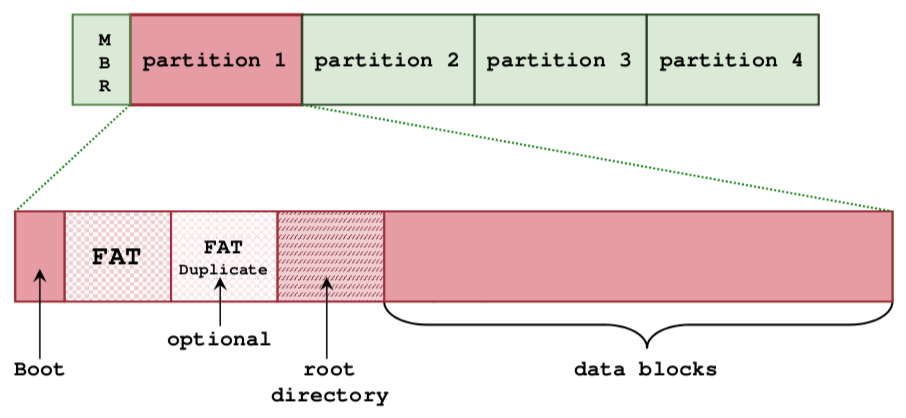
\includegraphics[width=\linewidth]{fatlayout}
  \begin{itemize}
    \item FAT12 -> FAT16 -> FAT32
    \item File data allocated to a number of data blocks/data block clusters
    \item Allocation info kept as a linked list, kept separately in the File Allocation Table (FAT) which is cached in RAM for linked list traversal: 1 entry per data block/cluster, store disk block information (FREE/EOF/BAD/next block number)
    \item Dir represented as special type of file
    \item Root dir is stored in a special location, other dirs are stored in the data blocks.
    \item Each file/subdir within the dir represented as \textbf{directory entry}
    \item Directory Entry 32-bytes, 8B+3B for file name+ext (first byte of file name may have special meaning: deleted, end of DE, parent dir, etc.), 1B for attributes, 10B reserved, 2B+2B for creation date+time (Year 1980-2107, time resolution $\pm2$ seconds), for the first disk block index (different variant diff number of bits, 12, 16, 32 for FAT12, FAT16, FAT32 respectively), 4B for file size in bytes.
  \end{itemize}
  \subsubsection{Accessing File/Dir}
  For a dir, disk blocks contain DE for files/subdirs within that dir
  \begin{enumerate}
    \item Use first disk block number stored in DE to find starting point
    \item Use FAT to find out subsequent disk block numbers
    \item Use disk block number to perform actual disk access on the data blocks.
  \end{enumerate}
  \subsubsection{File Deletion}
  \begin{enumerate}
    \item ``Delete'' the DE (set first letter in filename to \texttt{0xE5})
    \item Free data blocks: set FAT entries in linked list to FREE
  \end{enumerate}
  Do not keep track of free space information -- must be calculated by going through the FAT
  \subsubsection{Variants: FAT12, FAT16, FAT32}
  Support larger hard disk as a single partition
  \begin{itemize}
    \item \textbf{Disk cluster}: instead of using a single disk block as smallest alloc unit, use a number of contiguous disk blocks
    \item \textbf{Pros}: Larger cluster size -> larger usable partition
    \item \textbf{Cons}: Larger cluster size -> larger internal fragmentation
    \item On FAT32, further limitation: 32-bit sector count, only 28-bit used in disk block/cluster index.
    \item \textbf{Bigger FAT Size}
    \item e.g. 4KB cluster\\
          \begin{tabular}{| l | l | l |}
            FAT12                      & FAT16                       & FAT32                     \\ \hline
            $2^{12}$ clusters          & $2^{16}$ clusters           & $2^{28}$ clusters         \\
            4KB $\times 2^{12} = 16$MB & 4KB $\times 2^{16} = 256$MB & 4KB $\times 2^{28} = 1$TB \\
          \end{tabular}
    \item Actual size is a little lesser, special values (EOF, FREE, etc) reduces total number of valid data block/cluster indices.
  \end{itemize}
  \subsubsection{Long File Name Support}
  \begin{itemize}
    \item Virtual FAT (VFAT) supports long file names up to 255 chars
    \item Use multiple DE for a file with long filename.
    \item Use a previously invalid file attribute so non-VFAT will ignore these additional entries
    \item Use the first byte in the filename to indicate sequence
    \item Keep the 8+3 short version for backward compatibility
  \end{itemize}
  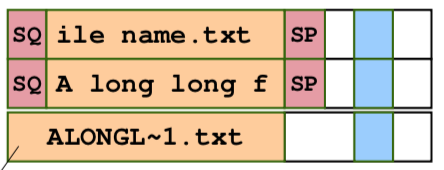
\includegraphics[width=0.6\linewidth]{vfat}
  \subsection{Extended-2 File System}
  \begin{itemize}
    \item Disk space split into \textbf{blocks}, blocks grouped into \textbf{Block Groups}
    \item Each file/dir is described by \textbf{I-Node} (Index Node) containing file metadata \& data block addresses
    \item For all bitmaps, 1 = Occupied, 0 = Free
  \end{itemize}
  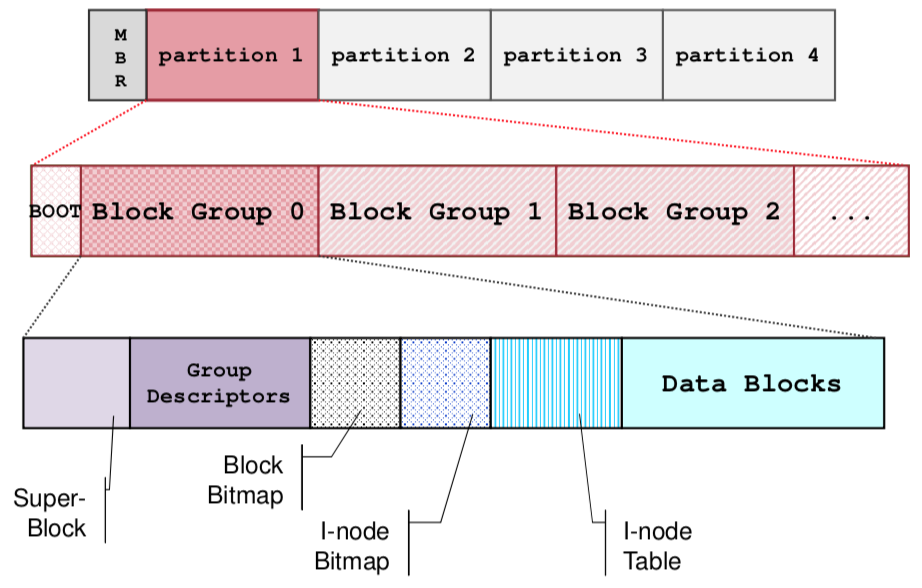
\includegraphics[width=\linewidth]{ext2layout}
  \subsubsection{Superblock}
  \begin{itemize}
    \item Describes the whole filesystem
    \item Duplicated in each block group for redundancy
    \item Includes total I-Nodes number, I-Nodes/group, total disk blocks, disk blocks/group, etc.
  \end{itemize}
  \subsubsection{Group Descriptors}
  \begin{itemize}
    \item Describes each of the block group -- no of free disk blocks, free I-nodes, location of the bitmaps
    \item Duplicated in each block group
  \end{itemize}
  \subsubsection{Block Bitmap}
  Keep track of the usage status of blocks of this block group
  \subsubsection{I-Node Bitmap}
  Keep track of the usage status of I-Nodes of this block group
  \subsubsection{I-Node Table}
  An array of I-Nodes, containing only I-Nodes of this block group
  \subsubsection{I-Node Structure (128 Bytes)}
  \begin{itemize}
    \item 2B for Mode: Filetype (regular, dir, special, etc) + File permission
    \item 2B user id, 2B group id
    \item 4B for file size in bytes, 8B for regular files
    \item 4B each for access, creation, modification, deletion timestamps
    \item 4B each for 15 data block pointers: 12 direct, 1 single indirect, 1 double indirect, 1 triple indirect
    \item 2B for refcount (no of times this I-Node is references by DE)
  \end{itemize}
  \subsubsection{I-Node Data Block}
  \begin{itemize}
    \item Allows fast access to small file, flexibility in handling huge file
    \item e.g. disk block address = 4B, each disk block is 1KB, so each indirect block can store $\frac{1\text{KB}}{4}=256$ addresses
    \item Max file size = direct + single indirect + double indirect + triple indirect = $12 \times 1$KB + $256 \times 1$KB + $256^2 \times 1$KB + $256^3 \times 1$KB = 12KB + 256KB + 64MB + 16GB = 16843020 KB
  \end{itemize}
  \subsubsection{Directory Structure}
  Data blocks of a dir store a linked list of DE for files/subdirs information within this dir
  \begin{itemize}
    \item I-Node number for that file/subdir (0 indicates unused DE)
    \item Size of this DE (to locate next DE)
    \item Length of the file/subdir name
    \item Type: File/subdir (or other special file type)
    \item File/subdir name (up to 255 chars)
  \end{itemize}
  \subsubsection{Accessing file/dir}
  \begin{enumerate}
    \item Root directory has a fixed I-Node (e.g. 2), read the actual I-Node
    \item Look at the next part in pathname, locate DE in current dir, retrieve I-Node number, read actual I-Node
    \item If dir, set current dir to this dir (read DE in pointed by I-Node)
    \item Else if a file, read content from blocks pointed by I-Node
  \end{enumerate}
  \subsubsection{File deletion}
  \begin{enumerate}
    \item Remove DE from parent dir (point prev entry to the next entry/end, if first entry, DE is replaced with blank record)
    \item Update I-Node bitmap (mark as free)
    \item Update block bitmap (mark as free)
  \end{enumerate}
  \subsubsection{Hard/Symbolic Link with I-Node}
  Dir A contains a file X, with I-Node\# N, dir B wants to share X
  \begin{itemize}
    \item \textbf{Hard Link}: creates a DE in B, using same I-Node\# N, can have diff filename. Increase refcount of I-Node\# N
    \item \textbf{Symbolic Link}: creates a new file Y in B, Y contains the pathname of X
  \end{itemize}

  \section{Additional Notes}
  \subsection{Internal vs External Fragmentation}
  \textbf{Internal fragmentation} is the wasted space within each allocated block
  because of rounding up from the actual requested allocation to the
  allocation granularity.

  \textbf{External fragmentation} is the various free
  spaced holes that are generated in either your memory or disk space.
  External fragmented blocks are available for allocation, but may be
  too small to be of any use.
\end{multicols*}
\end{document}
